\documentclass[a4paper]{article}

\usepackage[english]{babel}
\usepackage[utf8]{inputenc}
\usepackage{amsmath}
\usepackage{graphicx}
%\usepackage{tabu}
\usepackage{hyperref}
\usepackage{verbatim}
\usepackage{xcolor}
\usepackage{alltt}
%\usepackage{cleveref}

\title{Proposal}

\author{Roland Saur}

\date{\today}

\begin{document}

%\maketitle
\begin{titlepage}

\begin{center}


% Oberer Teil der Titelseite:

\includegraphics[width=0.15\textwidth]{tud.png}\\[1cm]    

\textsc{\LARGE Delft University of Technology}\\[1.5cm]

\textsc{\Large Thesis Proposal}\\[0.5cm]


% Title
\newcommand{\HRule}{\rule{\linewidth}{0.5mm}}
\HRule \\[0.4cm]
{ \huge \bfseries Distributed Software Agents in Smart Grids}\\[0.4cm]

\HRule \\[1.5cm]

% Author and supervisor
\begin{minipage}{0.4\textwidth}
\begin{flushleft} \large
\emph{Author:}\\
Roland \textsc{Saur}
\end{flushleft}
\end{minipage}
\hfill
\begin{minipage}{0.4\textwidth}
\begin{flushright} \large
\emph{Supervisors:} \\
Dr.~Amineh \textsc{Ghorbani} \\
Dr.~Igor \textsc{Nikolic} \\
Dr.~Martijn \textsc{Groenleer}
Prof.dr.ir. P.M. \textsc{Herder}  \\

\end{flushright}
\end{minipage}

\vfill

% Unterer Teil der Seite
{\large \today}

\end{center}

\end{titlepage}
\newpage
\tableofcontents
\newpage

\renewcommand{\abstractname}{Summary}
\begin{abstract}

\begin{comment}
\begin{figure}\includegraphics[width =\textwidth]{graphical_abstract.pdf}
\caption{Graphical Abstract}
\label{abstract}
\end{figure}
\end{comment}
Global warming is one of the main issues of the twenty-first century. The introduction of renewable energy sources (RES) and electric vehicles(EV) is promising, but poses a problem to the low voltage grid. \\
Smart grid technology can be used to manage and thus mitigate the negative effects RES and EVs have on the grid.
Smart grid technology to manage the low voltage grid not only deals with technical issues, but also has a social component. Smart gird technology should respect privacy, not ask for much user interaction and be widely accepted by users.\\
Most centralized approaches fail to achieve to comply with all the requirements. Distributed approaches seem promising but often need centralized management or infringe on the users privacy. If distributed solutions can be solve the management problem of low voltage grids and how they can coordinate their actions is the central question that arises.

\begin{comment}
A possible smart grid implementation that meets all the requirements is to use software agents, which have control over some appliances, like the charging of an electric vehicle. 
And since theses software agents appropriate a real and limited resource, in this case grid capacity, they contribute to the tragedy of the commons. 
In human systems the tragedy of the commons is averted by the introduction of Institutions.\\
The research question becomes whether or not the concept of Institutions can also be applied to a system with multiple agents when the agents are not human but software agents. 
\end{comment}

\end{abstract}
\newpage
\section{Introduction}
Carbon dioxide has become the main driver behind human made climate change, which poses a severe thread to society. The transport sector for now still relies mostly on oil. The switch to electrical vehicles although sensible, is only useful for reducing CO2 emissions if the electricity is generated by renewable energies. Unlike most other electricity sources, renewable energies are often integrated on the level of the low voltage grid.\\
Thus both electric vehicles and renewable energy sources(res) introduce massive changes in the, so far uncontrolled, low voltage grid. The grid not only has to be able to deal with the average load but more importantly the peak load that can occur within a day. Since PV production is dictated by the sun, PV production from distributed sources peak all at the same time and cause voltage peaks. The charging behavior of EVs is controlled by the owner of the car, however since most cars are used to commute to and from work, congested situation in which many people plug in their car at the same time, when they come home from work, can occur. For further increase of PV and EV in low voltage grids it might become necessary to reinforce the grid because of the increased peak loads.
The goal of smart grids is to manage the low voltage grid to redistribute load more broadly in time to have a lower peak load. The lower peak load means that the existing grid can handle a higher penetration of renewable energies and electric vehicles.  \\
In many smart grid solutions distributed intelligent agents and machine learning are being used. Distributed AI agents need some kind of reward function or goal for which to optimize. When it comes to reward mechanisms most research looks into using price structures to give an incentive to the agents to distribute their load to times when the price is lower.The overwhelming focus on monetary aspects has been criticized. Alternatively the grid could be seen as an common pool resource. This would mean that the reward function includes a direct feedback from the grid. This way the intelligent agent will have to strike a balance between charging the electric vehicle and not putting to much strain on the grid, instead of striking a balance between charging and cost. The rules about how and in which situation the grid constrains the behavior of the agents are set by the agents collectively through institutions. 
\\ \\
In the following chapter a short introduction into the term smart grids is given, followed by a collection of related research. After this my research approach will be explained with a short introduction into background information about Markov decision processes, Q-learning and the concept of artificial Institutions in common pool resource problems. Based on this the model design will be explained. 
In the end there will be a time line and a list of the exam committee. 


\subsection{Smart Grids}
The concept of smart grids is actually not very well defined. The term is more a problem description than a well defined concept. Most of the time it refers to the management of the production and consumption in the low voltage grid. \\ 
So far there was no need for managing the low voltage grid, since there was no production and the only demand was the average household electricity consumption. With the introduction of electric vehicles, the demand increases significantly and becomes less predictable. With the uptake of PV production the consumer becomes also a producer of energy and the low voltage grid is no longer just the place where electricity is consumed but also produced. The additional demand and production is in size comparable to the already existing demand. The easiest but also most expensive solution is to reinforce the low voltage grid to handle this new situation. It is much cheaper to manage this upcoming demand and production, than to reinforce the 
grid.\\
The problem research has to deal with is how to manage a smart grid. One of the simplest ways is to use demand response and price structures. Users get feedback about their energy consumption and the current price. This way they will get a feeling for how much energy they use and hopefully adapt their behavior. This is however not guarantied to work and has some privacy issues. \\

%The idea that smart grids could be mere monitoring systems providing feedback about electricity prices to bring people to change %their behavior and thereby distribute their consumption more broadly, is not just very unlikely to be helpful but also insulting to %humans by reducing them to simple money maximization machines.
% this is commented out so far
Managing the smart grid through software shows also some problems. Managing it centrally is tainted by a feeling of loss of control for the user and is computationally heavy. Distributed solutions work with AI agents, which make some decisions about when to switch on different household appliances or charge a backup battery or electric vehicle. However if agents work independently of each other they either fail to find an optimal solution for the overall grid or need some outside incentive.       



\subsection{Smart Grid Related Research}
This part is split into two research topics, the social aspect of smart grids and their technical implementation.\\ 
\subsubsection{Social aspects of Smart grids}
The social research is comprised of studies about acceptance of smart grids, management of smart grid through people called demand response, and the ethical problems that arise.
\cite{disgust1} points out that the main obstacle in implementing smart grids is that most users have a feeling of loss of control over their own appliances.\cite{disgust3} on the other hand shows that, while there is a concern over privacy and loss of control, it is outweighed once the user realizes the benefits of smart appliances.\\
Demand response is the idea that by giving feedback about pricing, households are more aware of energy and are thus steered towards a energy conserving lifestyle.\cite{disgust1} notes that by giving active feedback about the households energy consumption, the power consumption was reduced by 9\%. \cite{disgust2} talks about electricity consumption being contributed to lifestyle factors and that consumption can be reduced by "behavioral changes". The idea is that:"Technology and behavior thus have to complement each other."\cite{disgust2}. However others have raised moral concern about giving utility companies more power over appliances or giving them access to user data\cite{ethics1}\cite{ethics2}. The fear is that utility companies or smart home appliance manufacturer could misuse or sell data to third party companies, or use price structures "... to influence consumer energy usage behavior"\cite{ethics1}.  \\

%The thought that people are supposed to adapt their lifestyle to such a basic technology as electricity and that it should be ok to %monitor their daily life to find the best monetary incentive to influence their behavior, is at the very least missing the point that %technology should be means to an end and not the other way around and at the worst an affront to human dignity. 
% this sentence is not nice

\cite{smartcpr} points out that research in smart grids is often still stuck in a top-down centralized management way of thinking which 
might hinder the acceptance of smart grids in society, and proposes to view smart grids more like an common pool resource. People would be more willing to accept smart grids if 
they are actively involved in coming up with rules how to manage the grid and they can adapt smart charging schemes  to their needs. 
This would mean that the focus of research would change away from monetary incentives towards how to come up with rules to make the most of an existing infrastructure.Michael J. Sandel describes in his book ,"What Money can't buy" how monetary values can crowd out moral and ethical values and undermine community engagement in general. \cite{ethics2} has urged that ethical issues should not be features that can be added to existing smart grid concepts but rather central questions that should be addressed at the very beginning.
 \\
 \subsubsection{Technical aspects of smart grids}
Although research in the technical management of smart grids can have very different scopes, the overwhelming focus is on electricity and the aim is almost always the minimization of cost 
and the reduction of peak load. \cite{smartenergy} has pointed out that the focus on electricity might be too narrow-minded, and that a true smart gird would incorporate all kinds 
of energy. Although this point has validity, demanding smart grids that include heating and cooling of buildings might be premature since \cite{smartcpr} has pointed 
out that "smart grid" is still mostly a buzz word. \\
In the future one part of the smart grid will be a smart home. \cite{smarthome} explores the possibility of using particle swarm optimization to manage energy demands with 
distributed energy resources within one home.\\
More interesting than the management of one smart home is the management of the interaction between the smart homes, distributed energy resources and the electric vehicles(EV). 
The negative effect of electric vehicles(EV) can be mitigated by the use of smart charging or can even be beneficial to the grid through vehicle-to-grid operation(V2G). Smart charging sees 
the electric vehicles(EV) as a load that has to be managed to prevent higher peak loads. V2G views the battery in the EV as an active part of the grid. It can be charged when there 
is too much supply by PV and discharged when there is little to no PV supply present\cite{v2g}.\\
\subsubsection{Distributed Approaches to smart grid}
Most approaches to find smart charging or V2G schemes involve some kind of centralized management \cite{realtime}\cite{ACDC}\cite{eth}. \cite{realtime} points out that any real time
management of EV or smart grid has to be computationally inexpensive. In \cite{realtime} the smart charging is based on a price structure incentivising people to charge their EV at times 
when there is otherwise little load in the grid. This still requires the user to make an active choice about in which time zone he or she would like his/her EV to be charged. \\
\cite{eth} proposes a solution, while centrally managed acknowledges the EVs as autonomous agents within the grid. These agents report their utility autonomously. Which car gets to charge how much is then managed centrally based on the utility each individual car reported. The paper also 
mentions the possibility that agents could state incorrect values in order to seem more urgent to the system. In a congested situation in which there is too little capacity to satisfy
all of the demand each agent would state the highest value to maximize its share. This is analogous to common pool resource problems, the agents try to maximize their own utility with disregard for the other agents and thus exhaust the system.\\
\cite{reinforce_money} has introduced a truly distributed method to deal with smart charging, where every agent makes autonomous decisions, yet the combined peak load is reduced compared
to a uncontrolled charging scenario.
Such solutions are multi agent systems, composed of several agents. The agents decide about how much to charge the car on behalf of a person, without actual interaction with the person. In order for the agents to make an informed decision, they have to interact with the environment and find optimal strategies for charging. This is normally done by Q-learning. However, Q-learning does not always converge when used in a multi-agent system. 
Since each agent has a different reward function there is rarely a policy found which maximizes the benefits of all agents \cite{qfail}. Furthermore \cite{ai_cpr} points out that if the agents in multi agents systems appropriate a real and limited resource for humans, that the agents will contribute to the depletion of this resource if not properly restricted in their behavior. 

\cite{reinforce_money} solves this by making the reward,an agent gets, a combination of
utility gained from electricity usage, in household or through charging, and the cost of electricity usage.  Because the cost of electricity is in the reward
function, agents only charge up to a certain point, and it becomes more likely to charge when the price is low. This way the Q-learning algorithm in \cite{reinforce_money} distributes
the load more broadly over time and converges to a better solution than in the uncontrolled charging scenario. However the agent does not get rewarded for stabilizing the grid, it gets
rewarded for being most cost efficient, the positive effect for the peak load seems to be a side effect rather than the main goal of the research.  
This raises the question whether or not cost is the best indicator in the 
reward function to maximize the users benefit and the grids stability. On a broader perspective it raises the question how distributed AI systems, which do things on behalf of people should be managed. \\ 
\subsubsection{Research Problem}
In summary, the centrally controlled approaches to manage the low voltage grid fail to be responsive enough to deal with the fluctuating and changing nature of the low voltage grid and or infringe on the privacy of the user. Further make the feeling of loss of control and the privacy issues the uptake of such solutions rather unlikely. Distributed solutions have to be found to solve this very distributed problem. However most attempts at distributed solutions, need centralized management and or need to constantly communicate private data.



\subsection{Research Question}
The question to tackle is whether and how a decentralized approach can work in managing the smart grid. In order to answer this several sub-questions have to be addressed. 
\begin{enumerate}
\item Can a artificial agent representing a single household, without the input from a central management system be beneficial to grid stability?
\item How can multiple of  such household representing agents be coordinated in a decentralized way?
\item Can viewing the grid as a common pool resource and giving each household-agent the ability to contribute to the making of the rules and norms that govern the grid be beneficial to the overall grid stability? 
\end{enumerate}


\begin{comment}
The first is if a decentralized single household can without the help of a central management system contribute to the stability of the grid. The second question then becomes if multiple households each managed not centrally can overall benefit grid stability, if some rules are imposed on them. The third question is if viewing the grid as a common pool resource and giving each household the ability to contribute to the making of the rules and norms that govern the grid can be beneficial to the overall grid stability. 

In a very broad sense the research question deals with the problem of how to manage distributed AI agents, that appropriate a real resource. So there are software agents which use a real resource on behalf of people. This resource is finite and can be depleted by overuse. This is the tragedy of the commons, but the users are not human but software agents.\\ 
The research question becomes the question if the concept of institutions,which is normally applied to human systems, can also be applied to artificial systems.\\
The case that will be used to test this is smart charging algorithms in a smart grid. The finite resource is grid capacity and the agents are the smart charging algorithms.\\
In the following chapter the question of why to apply this to smart grids will be explained. Then some background on the software to simulate the grid, reinforcement learning, multi agent systems and artificial institution will be given. Afterwards the model will be explained and some experiment will be proposed.


\subsection{Benefits for Smart Grid}
A new smart grid concept has to respond to several issues, that have been explored in the related research section. The problems can be grouped in three topics, ethics, acceptance and technical. \\ 
The technical constraint are very easy to address instead of a central entity managing everything, each household gets its own software agent that manages smart appliances or backs up energy in a battery. These distributed AI agents would have to collaborate in some way to find a best solution for the whole grid. Some data has to be exchanged between them. This raises ethical problems about privacy and the autonomy of individuals. Thus only some data should be communicated. This limits the way the agents can collaborate. Agents cannot simply exchange electricity usage histories and come up with ideal strategies. However the concept of artificial institutions for artificial societies can be helpful. Artificial institutions are a set of rules that the agents themselves can vote on and each agent has to obey. The agents would then optimize their behavior under the constraint of artificial institutions and evaluate how well they are doing under the given set of rules. They then can vote again to change the rules in one way or another. The only information that has to be exchanged is the voting behavior, which says much less about the people living in the household than a complete history of electricity usage would.  This could also reduce the negative feelings of loss of control that people have, because no outside utility company has to or can interfere in the management. The focus would also be on community collaboration rather than money, which can further boost acceptance.     
%-Something about the general difference between what I do and what others did before.
\end{comment}
\subsubsection{Research Approach}
\subsubsection{Research methodology}
%here comes what I do to answer the different questions defined in the research question. 
In order to answer the research question a multi agent system has to be designed to intelligently manage the low voltage grid in a distributed way. 
The model will be represented by a markov decision process(MDP).\\
The environment of the MDP will be a low voltage grid. To have a realistic representation of a low voltage grid to work with, a low voltage grid has to be designed in theory, since there is no real grid information openly available. This theoretical grid then has to be transferred to a per unit model that can be interpreted by PYPOWER/MATPOWER. The agents in the MDP are software agents representing the different households. These software agents will control the charging and discharging of a battery. 
The state the agent is in is the SOC of the battery and the voltage at the grid point of the household.The action that the agent can take is to charge the EV at different rates within the next time step. This has an effect on the SOC and adds load to the grid point increasing the voltage deviation.  \\
\begin{comment}
The reward the agent receives is a function of the SOC of the battery and the voltage of the grid node. The higher the SOC the higher the reward, the higher the Voltage deviation from the norm the lower the reward.\\
\end{comment}
\begin{enumerate}
\item State\begin{enumerate}
\item SOC
\item Voltage
\end{enumerate}
\item Action\begin{enumerate}
\item Charge EV [0,5]kW
\item (Vote to change Reward function
\end{enumerate}
\begin{comment}
\item Reward\begin{enumerate}
\item $f(Voltage,SOC)=g(Voltage)+h(SOC)$
\end{enumerate}
\end{comment}
\end{enumerate}
\begin{comment}
The behavior of the software agents will be optimized to stabilize the grid, using Q-learning. This will be achieved by creating an interface between the machine learning software package pybrain and the PYPOWER.In order to have a basis on what to optimize different scenarios will be constructed based on changing load profiles at the different grid points. However not all data will be used, some data will be used for testing and evaluating, to have a scenario that the agents were not trained for.  \\
\end{comment}
Within the experiments the voltage at the different grid points and the state of charge of the batteries will be kept record of and evaluated using R.\\
\begin{comment}
Rules, that will be imposed on the agents, have to be designed in such a way that they have meaning in the context of Q-learning. This can either be in the form of a changed reward function to give incentive for specific actions or in the restriction of the action space from which the agents can choose their actions.\\  
\end{comment}

\subsubsection{Addressing Research Question}
To address the question an agent has to be designed, which can interact with the PYPOWER environment.
A graphical representation to better understand how the software agent is to interact with the grid,
can be seen in figure \ref{q1model}. This agent also has to have an internal policy to guide its behavior. 
The behavioral policy can be developed by the agent itself or can be imposed on the agent as an institutional
policy. The institutional policy is elected by all the agents collectively.  \\

\begin{figure}[!ht]
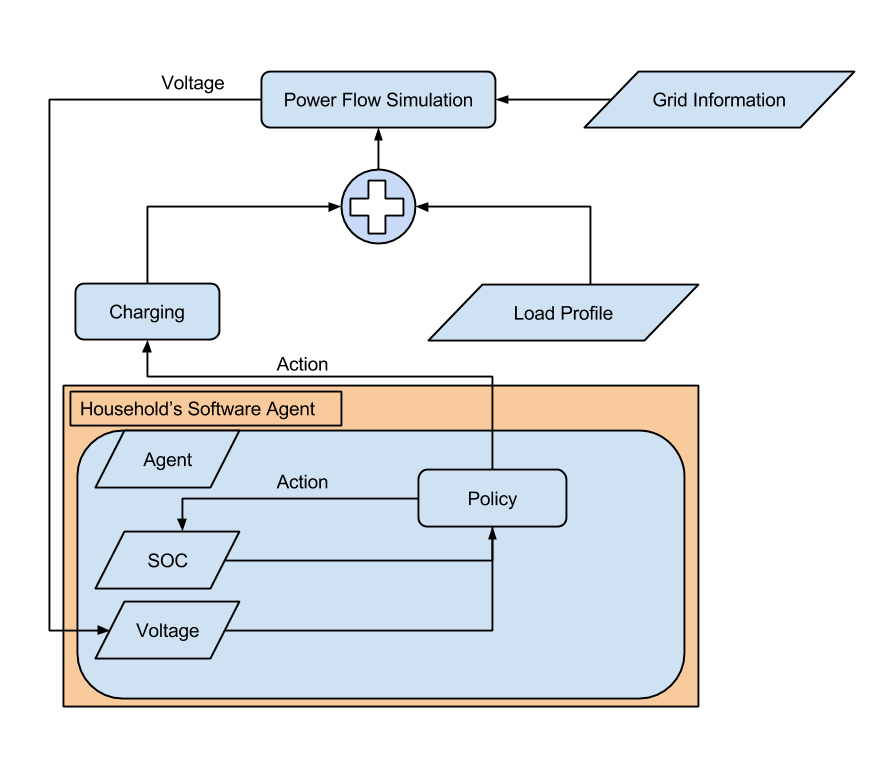
\includegraphics[width =\textwidth]{EV_smart_charging_model.png}
\caption{dsa}
\label{q1model}
\end{figure}

\begin{comment}
\subsubsection{Second Research Question}
To answer the second question the model has to be expanded to incorporate more than just one agent.\\
For this multiple agents have to access one PYPOWER model. For this a interface for more than one learner between pybrain and the PYPWOER/MATPOWER model has to be designed. \\
Similar to the single agent case the agents have to be trained given different load profiles to deal with. Then rules that restrict the agents behavior or give an incentive for specific behavior are introduced to the model. Due to the specifics of the Q-learning algorithm the rules imposed have to be tailored towards the Q-learning algorithm. \\ 
The resulting agent behavior will then be tested in different scenarios, that where not explicitly in the training data. The results will be judged by the ability to reduce voltage spikes in the grid overall. 
\subsubsection{Third  Research Question}
To address the third question the agents need to be able not just to abide by the rules but also shape those rules by interacting with one another.\\ 
In order to shape the rules there has to be a set of possible options on which the agents can collectively vote on. For this to be possible the agent first has to be able to judge different rules and rank them from least to most beneficial to the agent and the agents have to be able to communicate and reason with each other and come to an agreement.  An internal judging function for each agent and a voting mechanism to combine the votes into one solution has to be found. \\ 
To give the agents the ability to judge rules, a function to the existing agents has to be added. However in order to coordinate their voting behavior an additional agent has to be introduced. 
\end{comment}
\subsection{Research Tools}
\subsubsection{Powerflow simulation in MATPOWER/PYPOWER}
MATPOWER/PYPOWER is a software package for power flow simulations. MATPOWER/PYPOWER is available for Matlab, octave and python. The software package models AC and DC electrical networks. The inputs to the model are the network topology, given in a $n_b$x$n_b$ matrix, representing the impedance between the node points,  and the  $n_b$x$1$ complex load vector, representing the static loads at each node.  The model is then solved for the voltage and angle for each node. The model works internally by defining so called cases. Within these cases each node, Transformer and household is represented as bus, with its own bus index. The household usage of electricity is represented by P and Q values at the respective bus index. The lines between the nodes are defined in per unit values of impedance, active and reactive resistance. In order to transfer real impedance values of lines to per unit values, each case has a defined base voltag(Vbase) and power base(SBase). From these a base impedance can be calculated, see equation \ref{zbase}.\cite{powertransfer}
\begin{equation}
Z_{Base} = \frac{V_{Base}^2}{S_{Base}}
\label{zbase}
\end{equation}
Given the base impedance each line impedance can be transformed to per unit by dividing it by the base impedance, see equation \ref{zpu}.
\begin{equation}
Z_{pu}=\frac{Z}{Z_{Base}}
\label{zpu}
\end{equation}

Restrictions on the current that flows through the lines can be imposed. Further the model calculates how much energy has to generated by the generators, so that the only thing that has to be given is the load on the grid nodes.
\begin{comment}


\subsubsection{Reinforcement learning(RL) in Markov decision Processes}
A markov decision process is composed of discrete states $S_1,S_2,...S_N$. At each time step the system is in state $s_t=S_i$. There are transition probabilities from one state to another within one time step. These probabilities only depend on the current state,equation\ref{markov_prop}.This way the model does not have to keep track of everything that happened before but only what the current state of the system is.\cite{machine}\\
\begin{equation}
P(s_{t+1}=S_j| s_t=S_i,s_{t-1}=S_k,...s_1=S_{init})=P(s_{t+1}=S_j| s_t=S_i)
\label{markov_prop}
\end{equation}
In machine learning agents take an action $a_t \in A$ to change the state of the system $s_t \in S$. The environment rewards this new state with an reward $r_t \in R$.
\begin{figure}[!ht]
\includegraphics[width =\textwidth]{Machine_learning.pdf}
\caption{Agent environment interaction \cite{machine}}
\label{agent_machine}
\end{figure}
The agent then tries to find a policy $\pi$ that maps the state the agent is in to the action it should take($\pi: S \to A$).The agent will try to maximize the expected cumulative rewards and find an optimal policy. $Q(s_t,a_t)$ is the reward for taking an action $a_t$ in a state $s_t$. $Q^{*}(s_t,a_t)$ is the expected cumulative reward for taking action $a_t$ and then sticking to the policy $\pi$ for the rest of the system. The best policy can then be described as the policy that is composed of the actions with the maximum $Q^{*}(s_t,a_t)$.\\ 
The update rule is described by Bellmans equation, equation \ref{bellman}.$\gamma$ is a discount factor to discount future reward. \cite{machine}
\begin{equation}
Q(s_t,a_t)=E[r_{t+1}] + \gamma \sum_{s+1} \left(P(s_{t+1}| s_t,a_t)  \max_{a_{t+1}}Q(s_{t+1},a_{t+1})\right)
\label{bellman}
\end{equation}
 However most of the times even when the agent takes an action in a certain state the transition probability is unknown. The agent has to interact with the environment and learn the best result by trial and error. The agent has to take actions repeatedly and record the resulting states and rewards to update the reward $Q(s_t,a_t)$ that the agent expects to get by taking action $a_t$ in state $s_t$.\cite{machine}  
\begin{figure}[!ht]
\includegraphics[width =\textwidth]{Q-learning_algorithm.pdf}
\caption{Q-learning Algorithm \cite{machine}}
\label{q-learning}
\end{figure}
\end{comment}
\subsubsection{Multi Agent System}
Systems with more than one agent are called Multi Agent Systems(MAS)
If there are more than one agent, there are different ways of dealing with coordinating the learning between the different agents. The easiest way is independent learning, in which the agents simply ignore the other agents. Coupled learning is when each agent tries to model and estimate the effect of the others on the system. In specific cases in which all the agents share the same reward function, sparse cooperation can be used to combine all the agents to one agent.\cite{multiagent}\\
For agents to further cooperate in multi agent systems they can vote on mutual laws.  For this there has to be a set of options the agents can choose from and an internal function that ranks the different options. 
There are different voting mechanisms to combine the rankings the different agents made into one result. A simple majority vote takes the option that is most often chosen by the  agents to be the best option. A Borda count takes not just the highest ranked option into account but also the whole ranking of all options. Each agent attaches a number to the different options. The highest ranked option gets the number k-1 attached, while k being the number of options. The option below that gets k-2 attached and so on until the least favorable option gets 0 attached. The options then sum up all the values attached to them by the different agents. The option with the highest number then becomes the mutually agreed upon option.\cite{mas}

\subsubsection{Artificial Institutions}
This section will explain what a common pool resource(cpr) is, how institutions can help solve cpr problems and how the idea of institutions can be applied to multi agent systems. \\
Common pool resources(CPR) experience properties of both public and private
goods. \\
Similar to a public good, it is hard to exclude people from Common pool re-
sources. An example for this would be the atmosphere. It is impossible to
exclude people from the benefits of the atmosphere.
Similar to private goods the subtractability of common pool resources is very
high. The subtractability is not just how much value someone can extract from
the resource but also if this extraction affects the resource and how much others
can extract from it. This differs from a public good where the subtractability
is low. For instance Wikipedia would be a public good and not a CPR because
if you read an article on Wikipedia, it does not mean that others cannot read
the same article at the same time. The access to the internet, which makes
wikipedia possible, however is a common pool resource because if one person
uses up all the bandwith to Wikipedia, it would deprive others of their access to
Wikipedia.\cite{cprbook}\\
The problem of CPR results from these two properties. If an individual ex-
tracts value from the resource, the individual is the only one benefiting, yet the
negative effect of resource depletion is shared by everyone. This incentivises
individuals to extract as much as possible since their gain is greater than their
damage and if they do not extract as much as possible they would only experience the negative effects. The behavior is the rational behavior of an individual
but is irrational from a group perspective. This personally rational but group
wise irrational behavior is known as the tragedy of the commons.\\
The tragedy of the commons is often solved by using institutions. Institutions are  a set of rules and norms that all users in a 
system consent to. Rules need explicit, norms only implicit consent. By consenting to a set of rules, which restrict the user the 
commonly shared resource can be protected and it will not be depleted. This way the users can collectively arrive at a better situation 
than they could by individual reasoning\cite{institutions}. \\
\cite{ai_cpr} describes how software agents in real or virtual environments can experience the tragedy of the commons. Further software agents could autonomously appropriate a resource for a user. If these software agents do not cooperate or have rules to regulate their behavior they will contribute to the depletion of the resource. In human system a progressive tax on resource use is introduced to limit the users. The user only uses the resource up until the point when the tax burden outweighs the benefit\cite{ai_cpr}. An equivalent of such a tax mechanism for AI systems might be the reward function in Q-learning. It of course would not be in the form of money but in the form of an abstract negative reward for using the resource. The AI system would then use the resource until the reward it gains from the actual use outweighs the artificial negative reward introduced as an institution. 
\subsubsection{Borda count}
A majority voting system only takes into account the top choice of voters. The Borda count also takes into account second and third choices of voters, this way it is more representative of the actual preferences of the voters. \\
Lets say there are k candidates $\Omega = \{\Omega_1 , \Omega_2,\Omega_3,... \Omega_k\}$. The voters then rank those k candidates from most to least favorable. Weights will be attached to the different candidates in the following manner. The best candidate gets the weight (k-1), the second best (k-2) and so on until the worst candidate receives 0. The choice with the highest weight count gets selected as the winner of the vote.\cite{mas} \\
\subsubsection{k-means  Clustering}
The K-means clustering algorithm clusters n d-dimensional data points ,$x=\{ x_1,x_1,..., x_n\}$ into k clusters, $S_i$ with mean values $\mu_i$, so that the sum of square distances within the clusters is minimized. 
\begin{equation}
arg \min \sum_{i=1}^k \sum_{x \in S_i}\| x- \mu_i \|^2
\end{equation}
The algorithm consists of two steps which are repeated until the clusters no longer change. After initializing k centers of clusters randomly, all data points get assigned to their nearest cluster center. Then the cluster centers get updated by calculating the mean of all the data points in the cluster. 
\begin{figure}[!ht]
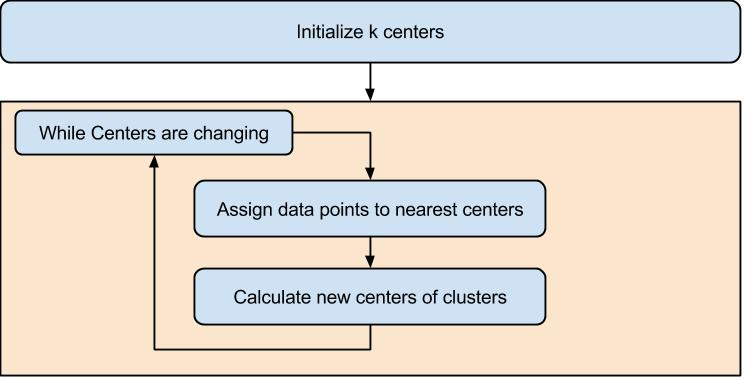
\includegraphics[width =\textwidth]{K-means_alg.jpg}
\caption{K-means Clustering Algorithm}
\label{k-means_picture}
\end{figure}

\newpage

\section{Problem description}
The integration of electric vehicles into the electricity grid poses opportunities and threats to stakeholders. 
The increase of electric vehicles can increase air quality in cities and the management of the load that 
EVs create can open up new markets for energy companies. The grid however might also not be equipped well enough to 
deal with the coming changes.\\
In the following two chapters the different stakeholders and their motivations are being presented and the reasons for 
this modeling approach are given.
\subsection{Stakeholders}
This chapter is based mainly on \cite{ev_stakeholder}. First the different stakeholders and how they perceive this 
transition to electric vehicles and then possible conflicts of interest are discussed.
\begin{enumerate}
 \item \textbf{Energy Companies:}\\
 To electricity companies the transition to electric vehicles is mostly an opportunity. It opens up a new market to them 
 in which they see the potential to charge different rates at different times to sell as much electricity as possible 
 at times when production costs are lowest due to excess renewable energy production. Further can the batteries in 
 electric vehicles be seen as cheap storage solutions for electricity companies. The main opportunity electricity 
 companies see in the introduction of EVs is to make it easier to balance the excess production of renewable energies
 and the peak load.
 \item \textbf{Grid operators:}\\
 Unlike electricity companies, grid operators are not allowed to sell electricity themselves and the transition is 
 therefore mostly a threat to them. While electricity companies are interested in making the peak electric load coincide
 with the production of cheap renewable energies to maximize their profits, grid operators are interested in spreading 
 the load more evenly to optimize use of the grid. Thus grid operators would prefer a more direct control over charging 
 strategies of electric vehicles. 
 \item \textbf{Municipalities:}\\
 Municipalities see the switch to EV as an opportunity to increase air quality, and thus switch their own fleets to 
 electric to be an example to others, and give financial incentives to further the introduction of electric vehicles. 
 \item \textbf{Consumer/Prosumer:}\\
 never ever gonna happen. 
\end{enumerate}
The main conflict between stakeholders is between energy companies and grid operators. This simply arises from the 
fact that the former uses the infrastructure and wants to maximize use of the infrastructure at times when it is 
most profitable to use it, and the later provides the infrastucture and wants to minimize investement in the infrastructure
and therefore the use to be as evenly as possible. This also causes the two parties to favor different solutions 
in the integration of electric vehicles. \\
grid operators more control, electritcity companies more flexibility in use and price structures. 

\subsection{Why Modeling/Modeling approach}
The stakeholders problem is situated in a socio-technical system including, almost every aspect of peoples daily life, 
since electricity is ubiquitous, and expensive infrastructure, the electricity grid. This makes experimenting to find 
best solutions, very difficult, because failures could have very adverse affects on peoples lives and therefore on the 
reputation of the concept of smart grids. Possible failures could also cause damage to infrastructure which would not just
be disruptive but also expensive. System obviosily have to be tested at some point in real world scenarios. But it is 
very important to have a good theoretical understanding of how the system could possibly behave in reality. Therefore 
models have to be deviced, which are most accurate representations of the socio-tehcnical system and the 
software solution that is proposed to solve the problem. \\
The model has to consist of a physical layer representing the grid and a multi agent system to represent peoples 
behavior and the software agents choices. The first step in solving the problem in this theoretical model is 
to check if the model experiences the initial problem in the way predicted. For this each household is given a 
software agent, and behavior of the software agents is set to charge as long as the battery is not at 100\% charge,
at the highest possible rate.\\
The result of such a test are given in graph \ref{software_tragedy}. In this graph the state of charge over time is 
represented for different levels. the level in this case is an indication of how close or far from the 
electricity source the electric vehicle is situated. The higher the level the further the EV is from the source. 
What we can see is that the state of charge for EVs on level 5 and 6 are not able to recover to full charge after being 
drained. They sometimes even drop down to 0, meaning completely empty. This is the abstract 
representation of the tragedy of the commons in the smart grid with a lot of EVs accessing the grid. Some agents 
cannot access the resource, the grid, because it has been depleted by the self interest driven actions of 
all of them. This way the model represents the initial problem of too many electric vehicles charging at the same time 
and overloading the grid. 


\begin{figure}[!ht]
 \centering
 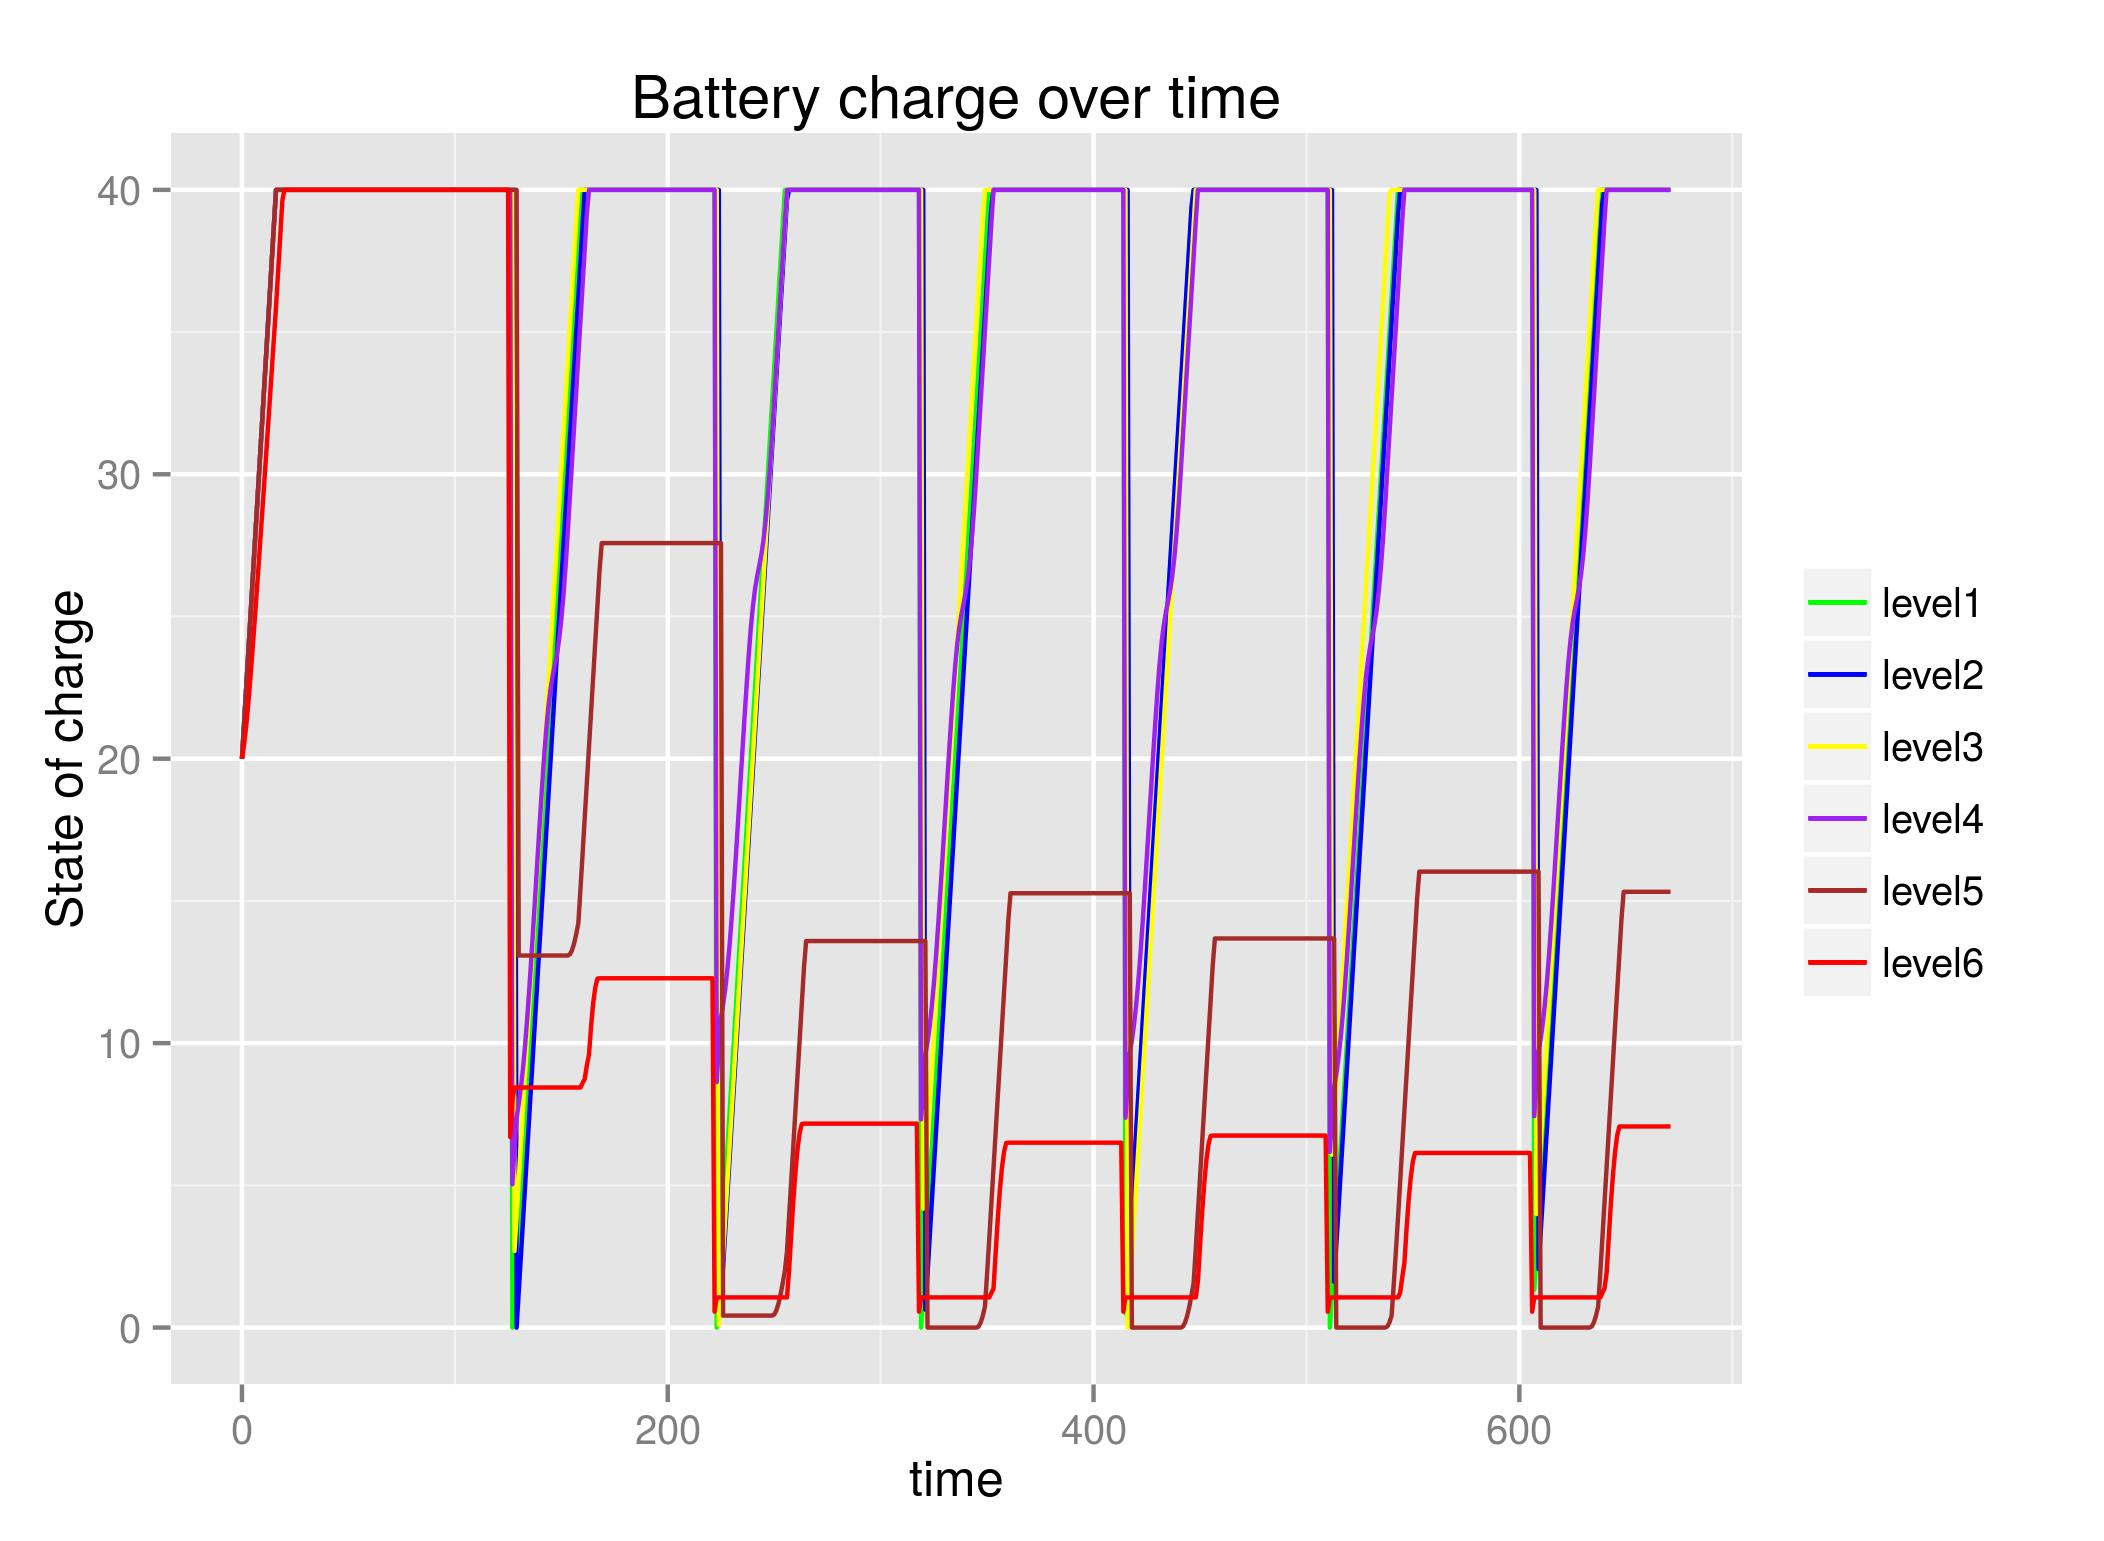
\includegraphics[width = \textwidth]{tragedy_of_commons.jpg}
 \caption{Tragedy of the commons in the Model}
 \label{software_tragedy}
\end{figure}

\clearpage

\section{Model}
\subsection{Concept}
First the components of the model will be explained. Then a overview of the processes that the agents go through will be 
given. The agents, how their rules and memory work and how the agents come up with rules collectively through voting 
will be explained afterwards.
\subsubsection{Model components}
The model consists of three parts , a physical layer represented by the Matpower model, software agents and an institutional 
layer, which sets the norms. 
The main active part in the model are the software agents. They interact with the physical layer by requesting a 
specific amount of power from the grid and receiving feedback about how much power they actually get. They also vote on rules 
and follow institutional rules as active rules. 
Agents have physical attributes, such as Battery , a node position and the corresponding voltage,  which determine their 
place in the real world. The agents make decisions based on their rules. Their preference, memory and connections to others 
are used to come up with and vote on new rules.
\begin{figure}[!ht]
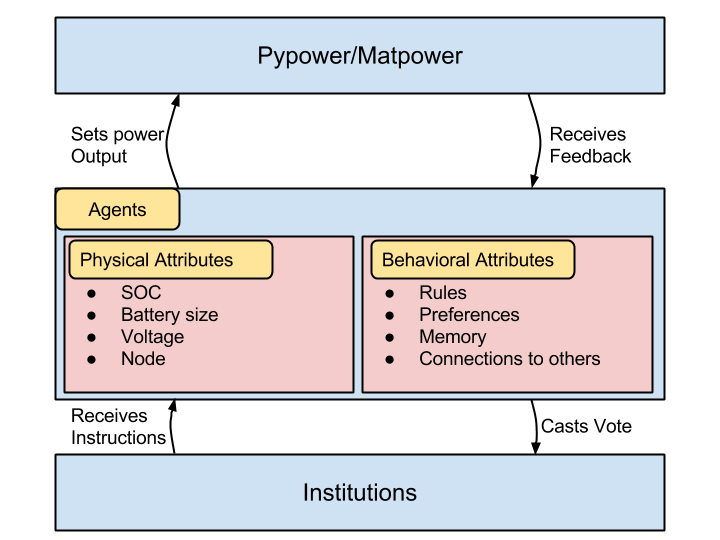
\includegraphics[width =\textwidth]{concept_components.png}
\caption{Model components}
\label{mcomponents}
\end{figure}

\subsubsection{Agent gets up drinks a cup of coffee}
Each agent goes through the following process, depicted below. For one week in intervals of 15 minutes, the agent 
chooses an action based on their internal rule. The matpower model then calculates a feedback which the agents internalize
by updating their voltage and state of charge. Each week the agent evaluates the rule it has been living with based on how 
high their battery state of charge over this past week was, and commits the rule and an associated preference value to 
its memory. Afterwards the agent comes up with a new rule for the next week. When the memory of the agents is not yet 
filled the agents develop the rules themselves. Voting is also omitted when a rule that has been voted on, was not good 
enough to be in at least a certain percentage of the agents memories. This percentage is called the institutional success 
rate. For the voting the agents report their ranked memory. The vote itself is done by borda count and then clustered.  
The agent can come up with a new rule by either learning based on their memory, copying from the best performing other 
agent or randomly selecting a new rule. The new rule is then set as the new active rule in the agent, and the process is
started over again.
\begin{figure}[!ht]
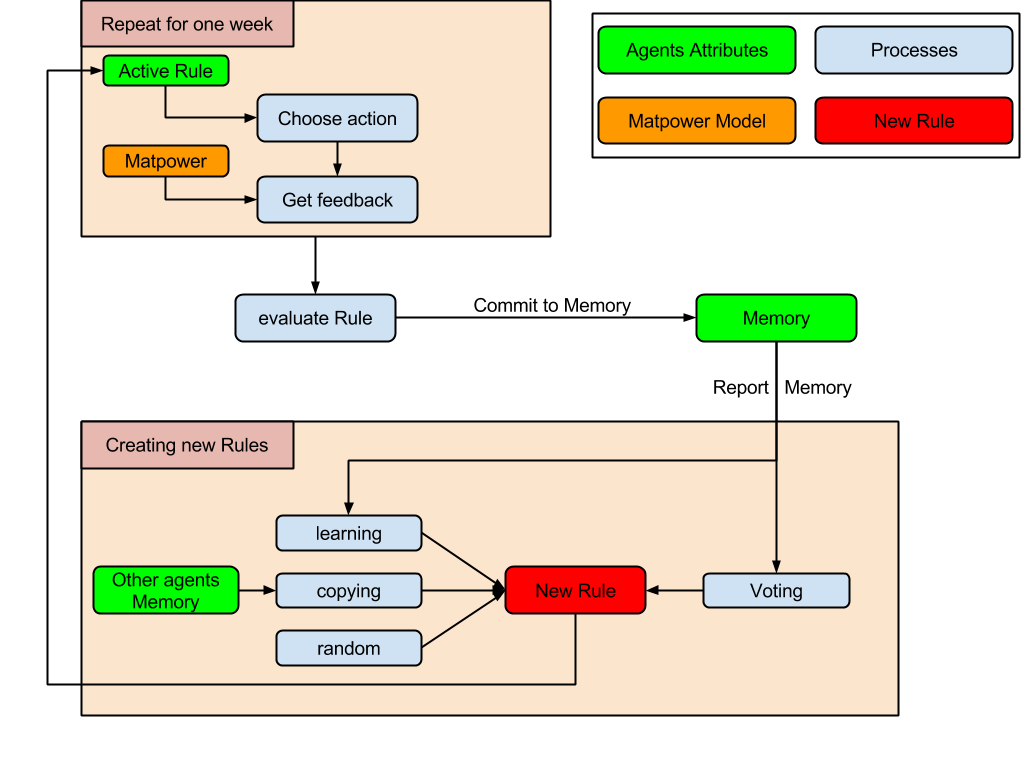
\includegraphics[width =\textwidth]{concept_coffe.png}
\caption{Model processes}
\label{model_coffee}
\end{figure}

\subsubsection{Rules}
Rules in the agents govern their behavior. They return a corresponding action given a specific state. The state of
an agent is its state of charge(SOC), the voltage at its node and the current time. Rules basically map a specific 
combination of these variables to an action. The action is how much the agent will charge in the next time step. 
\begin{figure}[!ht]
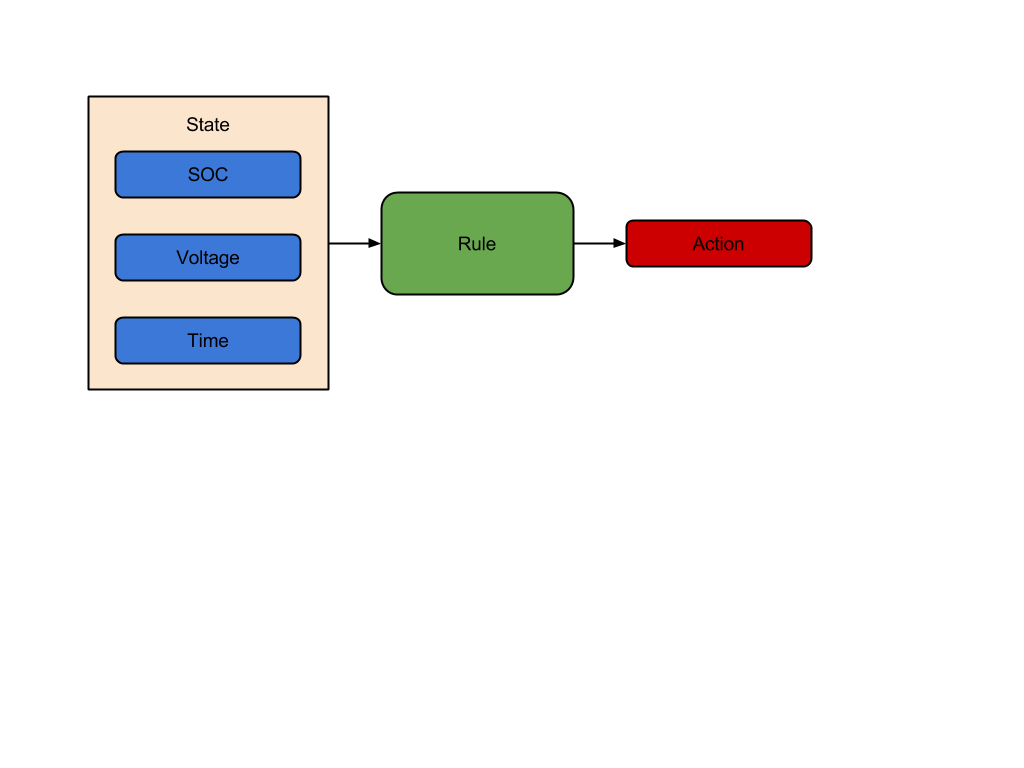
\includegraphics[width =\textwidth]{concept_rules_function.png}
\caption{The function of rules}
\label{rules_function}
\end{figure}

Rules can either be based on the current time and state of charge(soc) or on the voltage at the grid point and 
the state of charge(soc). Voltage bases rules are indicated with a 1 and time based rules are indicated by a 2.

\begin{figure}[!ht]
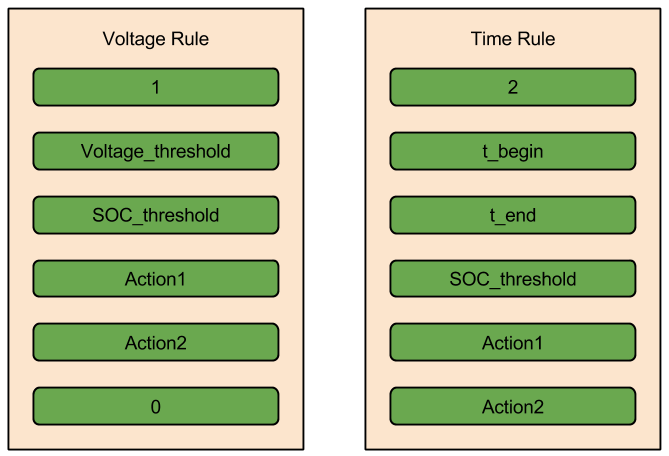
\includegraphics[width =\textwidth]{concept_rules_structure.png}
\caption{The structure of rules}
\label{rules_structure}
\end{figure}

A voltage rule has a voltage and a state of charge threshold and two actions - action1 and action2. 
If the voltage of the agent is below  the voltage threshold defined in the rule and its state of charge is above 
the minimum state of charge defined in the rule, the agent decides to take action1. If this condition is not true the 
agent takes action2. 
Voltage rule: (State=Blue, Condition = Green, Action = Red) \\ 
\begin{alltt}
If (\textcolor{blue}{Voltage} < \textcolor{green}{Voltage_threshold}) & (\textcolor{blue}{SOC} > \textcolor{green}{SOC_threshold})
    then do \textcolor{red}{Action1} 
else 
    do \textcolor{red}{Action2} 
\end{alltt}

A time rule has a similar structure. It contains two times, $t_{begin}$ and $t_{end}$, to define a time interval and 
a minimum state of charge ($soc_{threshold}$). If the agents state of charge is above the minimum, defined in the rule, 
and the time is within the specified time interval the agent takes action1, otherwise the agent takes action2. 
Time rule: \\ 
\begin{alltt}
If (\textcolor{green}{time_end} < \textcolor{blue}{Time} < \textcolor{green}{time_end}) & (\textcolor{blue}{SOC} > \textcolor{green}{SOC_threshold}) 
    then do \textcolor{red}{Action1} 
else 
    do \textcolor{red}{Action2} 
\end{alltt}

\subsubsection{Memory}
Each agent has a memory to keep track of past rules and how good the agent thinks this rule was. The memory 
is needed for the learning and for being able to vote. The memory consist of 5 past rules and associated preference 
values. The rules are kept in memory based on merit.
Each time an agent commits a rule to its memory, it calculates the average state of charge of its battery under this rule. 
This value is the preference value for this rule. If the rule is already in the memory the preference value becomes the 
average of the two preference values. If the rule is new it replaces the worst rule in the memory if its preference value 
is higher than the preference value of the worst rule in memory. Afterwards the memory gets sorted from best to worst. 

\begin{figure}[!ht]
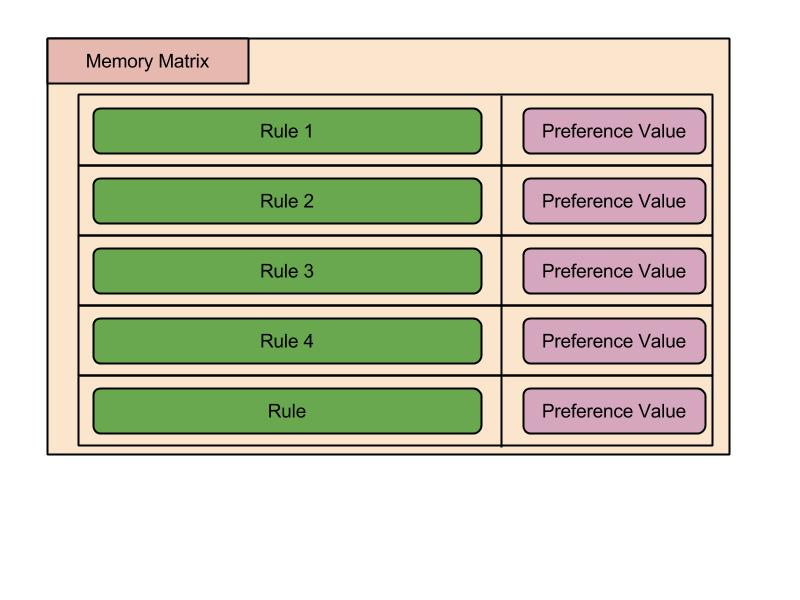
\includegraphics[width =\textwidth]{concept_memory.jpg}
\caption{The structure of Memory in the agents}
\label{Memory_structure}
\end{figure}


\subsubsection{Voting}
The agents report their memory as a vote. Borda count is used to duplicate the rules in the matrices based on their rank. 
The top ranked rule in one memory matrix will be duplicated 4 times, the second best rule in the matrix will be duplicated 3
times and so on. Duplicated this way the votes are then all combined into one election matrix. The decision whether a new rule
should have a voltage or time condition can be made by simple majority vote. The specifics of the conditions will be 
determined by clustering the rules into 3 clusters. The center of the cluster containing the most votes will be used as 
the specific condition for the rule.


\subsubsection{Model assumptions and choices}

\begin{enumerate}
 \item \textbf{General assumptions} \begin{enumerate}
                            \item \textbf{The global time is kept track of by the ticks. One tick is 15 minutes} \\
			     To make it easier to keep track of the time of day the model always starts at midnight. 
			     This way the modulo of the global tick by 96 indicates the time within the day.
			    \item \textbf{The agents can either be at home or not at home. The mean arrival/leaving times of 
			    all the agents are gaussian distributed. The mean battery drain of all the agents is 
			    gaussian distributed with mean equal to the average battery drain.} \\
			    Given the central limit theorem the assumption that the mean of a variable over multiple agents is 
			    gaussian distributed  means that  the variable has the same distribution for each agent.
			    \item \textbf{Power consumption exceeding this voltage level will be capped. } \\
			    The agents have to get feedback from the MATPOWER/PYPOWER model. In order for this to happen current 
			    and or voltage constraints have to be imposed on the model. Based on the maximum current in one
			    line the maximum voltage that can appear can be derived. 
                           \end{enumerate}
 \item \textbf{Assumptions/Choices  about Rules} \begin{enumerate}
                                         \item \textbf{The number of rules that dictate the behavior of the agents will be 
                                         fixed to one rule} \\
                                         Otherwise a meta rule is needed to decide which rule should be used. 
					 The one rule has to give an action in any possible situation. Not charging is still
					 an action. This means the rule will be a if-else structure with 2 actions , 
					 an action which will be executed when the condition is fulfilled and one default 
					 action.
					 The condition in the rule can only be dependent on variables the agent can observe - 
					 its SOC, Voltage and the time. Since the state of charge is the main interest of the
					 agent it should always be in the rule. Two kinds of rules, soc-time-condition and 
					 soc-voltage-condition, will be possible.
					 \item \textbf{Each agent keeps  5 previous rules and corresponding preference 
					 values in memory }\\
					 For simplicity sake the number of rules is kept fixed over time.
					 
					 \end{enumerate}
					 
\item \textbf{Assumptions/Choices  about voting} \begin{enumerate}
                                         \item \textbf{Borda count will be used for the voting} \\
                                         The voting mechanism should find the solution that is most prefered by all 
                                         the agents. Simple majority rule often fails to do this. Borda count makes the 
                                         voting more representative of the actual preferences of the agents. 
                                         \item \textbf{K-means clustering algorithm will be used to cluster the 
                                         rules into 3 clusters} \\
                                         Since there are too many possible rules and too few agents to vote on them, simply 
                                         counting will fail. Very similar rules would be counted as completely different rules. 
                                         This issue will be fixed by clustering the rules into several clusters of rules. 
                                         The k-means algorithm needs  the number of clusters as input to be fixed.
                                         \item \textbf{Agents cannot vote and come up with rules at the same time} \\
                                         In order for agents to vote they need to be able to rank their choices from worst 
                                         to best. This ranking can only happen if the agents can evaluate the choices with 
                                         some metric. This evaluation can either come from experiencing the rule and 
                                         observing how well the agent performs under this rule or by a fixed evaluation 
                                         function. An evaluation function can only work if the agent can beforehand 
                                         estimate the effects of a rule on their performance. Since there are several 
                                         agents interacting, estimating beforehand the effect of a rule is unlikely to work. 
                                         This means that in order to give a meaningful preference value to a rule the rule 
                                         has to be experienced. Agents can only evaluate and thus vote on  the rules that 
                                         they have followed in the past. 
                                         \item \textbf{Voting will be omitted for one week if the institutional rule 
                                         is not good enough} \\
                                         Once the initial exploration phase is over and the agents have filled their memory 
                                         and the voting has begun, the set of possible rules the agents can come up with by 
                                         voting is limited.  If a rule has been voted on and this rule then performs very 
                                         poorly it might be because the set of rules it was selected from was too limited 
                                         to contain a good solution. It would then only be reasonable to let the agents 
                                         explore the complete set of rules again to expand the set of possible rules. 
                                         \item \textbf{The first five weeks the agents only develop the rules themselves }\\
                                         This is just  to fill their memory. The voting with borda count makes very little
                                         sense if there are only one or two rules in the memory to be ranked.




                                        \end{enumerate}


\end{enumerate}


\subsection{Implementation}
The model was written in Pyhton because the language is easy to use and has a full implementation of MATPOWER, called
PYPOWER, and the k-means algorithm. A detailed description of the model implementation and pseudo 
code can be found in Appendix C . 
\subsection{Verification}
Two parts of the model have to be verified. That the multiagent system itself works and that the PYPOWER model 
represents reality in the intended way.\\
For the multiagent system, the agents individual behavior and their collective behavior, interacting with each other was 
tested. For the PYPOWER model the constrain mechanism was tested.\\
An extensive list of all the tests that were done can be found in Appendix B. 

\newpage

\section{Experimental}
\subsection{Basic setup}
In this chapter the basic experimental setup will be explained. First the input, that is needed to run the model 
and the time frame for the model is stated. Then the data that will generally be output by the model will be explained 
and finally how this output will be interpreted will be explained. 
\subsubsection{Input}
Each run of the model will consist of six months of simulation in 15 minute intervals. The global variables that are fixed
over all the experiments and have to be provided are the following. 
\begin{enumerate}
 \item \begin{alltt}time\end{alltt}
 \item \begin{alltt}average_arrival_time = 72 (6pm)\end{alltt}
 \item \begin{alltt}average_leaving_time = 32 (8am) \end{alltt}
 \item \begin{alltt}sd_average = 1 (quarter of an hour)\end{alltt}
 \item \begin{alltt}average_battery_drain = 10 \end{alltt}
 \item \begin{alltt}sd_average_battery_drain = 2\end{alltt}
 \item \begin{alltt}average_soc = 20 \end{alltt}
 \item \begin{alltt}sd_average_soc 2\end{alltt}
 \item \begin{alltt}soc_max_gloabl = 40\end{alltt}
 \item \begin{alltt}action_options = [0,1,2,3,4,5]\end{alltt}
 \item \begin{alltt}t_begin_options = [1,2,.....,96]\end{alltt}
 \item \begin{alltt}t_end_options = [1,2,.....,96]\end{alltt}
 \item \begin{alltt}soc_threshold_options = [  0.,   5.,  10.,  15.,  20.,  25.,  30.,  35.,  40.]\end{alltt}
 \item \begin{alltt}voltage_options = [ 0.96,  0.97,  0.98,  0.99,  1.  ]\end{alltt}
\end{enumerate}

There are other global variables which will be initialized to an empty value but will emerge from the model.
\begin{enumerate}
 \item \begin{alltt}institutional_rule\end{alltt}
\end{enumerate}

There are also global variables which will be defined within the specific experiments and are therefore mentioned later in the experimental part. Those variables mostly deal 
with how the agents come up with rules and how they vote on rules. 
\begin{enumerate}
 \item \begin{alltt}random_change\end{alltt}
 \item \begin{alltt}copy_best_change\end{alltt}
 \item \begin{alltt}learn_change\end{alltt}
 \item \begin{alltt}institutional_success_rate\end{alltt}
 \item \begin{alltt}copy_all\end{alltt}
 \item \begin{alltt}majority_vote\end{alltt}
\end{enumerate}

\subsubsection{Output}
The output of each experiment is written to a comma separated files(.csv).To evaluate the different runs the following 
variables are written to the output file for each time step. \\
To keep track of time and to identify each run. 
\begin{enumerate}
 \item run\_id
 \item time
\end{enumerate}

Part of the output of each experiment has to be the the input variables that defined the exact experiment.
\begin{enumerate}
 \item random\_change
 \item copy\_best\_change
 \item learn\_change
 \item copy\_all
 \item institutional\_success\_rate
 \item majority\_vote
\end{enumerate}

The output is also  defined by the question that needs to be answered. What is of interest in the model is how and 
if the model solves the common pool resource problem. The tragedy of the commons in this case is that some agents are 
not able to charge sufficiently. Therefore the state of charge of the battery is kept track of for each agent.
\begin{enumerate}
 \item agent1\_soc
 \item ...
 \item agent24\_soc
\end{enumerate}

The institutional rule, how quickly it changes over time and how frequently it fails gives insight into how the 
agents try to solve the tragedy of the commons. The institutional rule is split in its 6 parts to make it easier to write
to and read from the output file. 
\begin{enumerate}
 \item institutional\_rule = [inst\_rule1,... inst\_rule6]
 \item voting
\end{enumerate}

The exact structure of the output and how it will be done in detail will be explained in the appendix.

\subsection{Performance indicators}
The output will be evaluated using the statistical tool R. In this section the properties which are desirable 
are quickly explained and then a list of performance indicators, that help in looking for these properties is given.\\
The model is only useful if the agents find a stable solution. If the agents cannot find a rule ,which they agree on,
the results will fluctuate in between weeks and the agents do not work reliably. Ideally the agents would vote on an 
institutional rule after an initial phase of exploration and then only make minor changes to the rule so that 
the results stay similar over the following weeks.\\
\begin{enumerate}
 \item \textbf{stability:}\\
 How often the \textit{voting} variable indicating if the agents currently vote or explore, changes within the last 
 two months of the model run. 
\end{enumerate}

Secondly the model describes a common pool resource, therefore looking at the average performance of the agents 
is not useful for judging if the agents solved the cpr problem. Therefore the focus has to be on the weakest agent 
in the model. Looking at the average state of charge of the weakest agent in the model is an indicator of 
how well it performs but this is however still a blunt tool. It is better to define events within the model which relate 
to the real world of electric vehicles. An event like ,an agent not being able to fully charge the electric vehicle 
within one week or an agent not being able to charge the electric vehicle sufficiently, 
meaning that the state of charge of its battery drops to zero, is an event that has meaning in the real world and can 
be identified in the model output. Further it can also be said that an agent not being able to charge sufficiently is a
much worse event than an agent not being able to charge to 100\%.
\begin{enumerate}
 \item \textbf{Average SOC:}\\
 Average state of charge of the weakest agent in situations when there is an institutional rule in place.
 \item \textbf{Frequency of weak failures:}\\
 How often in one run it occurs that 
 an agent cannot charge to 100 \% in a situations when there is an institutional rule in place.
 \item \textbf{Frequency of hard failures:}\\
 How often in one run it occurs that 
 an agents state of charge drops to 0 in a situations when there is an institutional rule in place.
\end{enumerate}


\begin{comment}
There are some basic statistics that will be used , such as the mean, median and spread of variables.
More interesting is how the state of charge of all the agents will be used to interpret a model run or a specific
rule as a success or failure. Simply looking at the mean state of charge over all the agents is not sufficient 
to indicate if some agent failed.  In particular the state of charge of the agents which in the unconstrained test 
had the lowest average state of charge are of most interest. If a rule itself is a failure will therefore be judged
by how the state of charge changed over a week. If the state of charge for the weakest agent never reaches 100\%
it is considered a “weak failure”. If the state of charge for the weakest agent drops to 0 it is considered a 
“strong failure”, because it indicates that there was not enough time to recharge the battery to a needed minimum. 
The graph below depicts a weak and strong failure. The brown line depicts the state of charge of an agent on level 5.
The agent shown by the brown line has a higher average state of charge than the agent shown by the red line.
However the agent on level 6 is arguably doing better, because its state of charge never drops to 0, meaning 
that there is always sufficient charge in the battery  to commute to and from work. The model setup is 
considered a failure based on the frequency of failure of the institutional rules.
\end{comment}

\subsection{Hypotheses}
\begin{enumerate}
 \item \textbf{Behavioral Hypotheses} \begin{enumerate}
                                       \item \textbf{By increase the copying behavior the model performs worse}\\
                                       Rules are evaluated by each agent individually. Rules which are best for the 
                                       individual are bad for the system as a whole. Those rules are problematic.
                                       When more agents copy the rules from the best performing agent these problematic 
                                       rules become more prevalent and thus the model performs worse.
                                       \item \textbf{By increasing the learning behavior the model performs worse} \\
                                       By learning the agents only interpolate their memory but not extrapolate to new rules.
                                       This way the span of rules within the agents gets limited and thus also the overall 
                                       pool of rules is limited. A limited set of rules makes it harder to find overall 
                                       good rules and thus the performance of the model will suffer. 
                                      \end{enumerate}
 \item \textbf{Institutional Hypotheses} \begin{enumerate}
					  \item \textbf{The model performs better when using borda count compared to 
					  majority voting.}\\
					   Majority voting only takes the top ranked rule of each agent into account. 
					   Borda count takes a ranked list of rules into account and is therefore more 
					   representative of the actual preferences of the agents. This way rules which 
					   are not best for most but good for all are more likely to be elected and thus
					   the model performs better. 
					  \item \textbf{A high institutional success rate makes the model unstable.}\\
					  The institutional success rate is the percentage of agents which have to be satisfied 
					  by an institutional rule to continue the voting. If the percentage becomes too high 
					  no rules will be able to be good enough. The model will jump between institutional 
					  and personal rule and not be stable.
					  \item \textbf{A low institutional success rate makes the model perform worse.}\\
					  The institutional success rate is the percentage of agents which have to be satisfied by 
					  an institutional rule to continue the voting.  If this rate is too low the model will 
					  continue voting even if the set of rules to vote on is too limited to come
					  up with an adequate solution. The model will perform worse because what is 
					  seen as satisfactory is set too low. 
					  \item \textbf{Majority voting fails to overcome  a greedy rule.}\\
					  If a greedy rule, charge as much as you can whenever you want, is already 
					  introduced to the system as an institutional rule, there is a certain proportion
					  of the agents which will vote for this rule, because of their advantaged situation.
					  In simple majority voting it is very unlikely that a bigger group of agents
					  can agree on one rule to favor, than are already in favor of the greedy
					  rule simply by their position.
					  \item \textbf{Borda count can overcome a greedy rule.} \\
					  If a greedy rule, charge as much as you can whenever you want, is already 
					  introduced to the system as an institutional rule, there is a certain proportion
					  of the agents which will vote for this rule, because of their advantaged situation.
					  Unlike majority voting, borda count merely needs most agents being content with
					  a rule to make it an institutional rule.
					  \end{enumerate}
\item \textbf{Neighborhood Hypotheses} \begin{enumerate}
                                        \item \textbf{Grouping agents in neighborhoods  improves the performance of the model.}\\
                                        Rules are evaluated by each agent individually. Rules which are best for 
                                        the individual are bad for the system as a whole. Those rules are problematic.
                                        Problematic rules can spread through the set of agents by copying. Grouping the
                                        agents into neighborhoods contains problematic rules to the neighborhood, which
                                        makes them less likely to become institutional rules and thus improves performance.
                                        \item \textbf{Vertical grouping creates better results than horizontal grouping.}\\
                                        Rules are evaluated by each agent individually. Rules which are best for the 
                                        individual are bad for the system as a whole. Those rules are problematic. 
                                        Problematic rules can spread through the set of agents by copying. 
                                        Horizontal grouping is grouping the agents which are most alike in one 
                                        neighborhood. Those who are closest to the source get grouped in one 
                                        neighborhood and those who are furthest away from the source get grouped 
                                        into another neighborhood. Horizontal grouping results in homogeneous groups. 
                                        Problematic rules can spread more easily in homogeneous than in heterogeneous
                                        groups, therefore horizontal grouping will create worse outcomes because of 
                                        more homogeneous neighborhoods. 
                                       \end{enumerate}
\item \textbf{Contextual Hypotheses} \begin{enumerate}
                                      \item \textbf{Emerging rules are only functioning in the particular infrastructure 
                                      they emerged in.} \\
                                      Even small changes in infrastructure have a significant influence on how
                                      a load is affecting the voltage on a grid point. This has an effect on
                                      whose demand is getting cut and therefore on how the different agents 
                                      perform in the model. So rules which work in one setting, may creating 
                                      bottlenecks in other setting.
                                      \item \textbf{Increasing the variance in base load results in more random rules.} \\
                                      Randomness in the base load affects the effect a rule has on the performance 
                                      of the agent and increases therefore the potential difference between how good
                                      the rule is and how good the agent thinks the rule is. If the variance in
                                      the base load is increased the evaluation of rules becomes less based on
                                      merit and more random. If the evaluation of the rules by agents becomes 
                                      random the rules that get elected also become more and more random.
                                     \end{enumerate}
\end{enumerate}

\subsection{Experiments}
In this chapter the experiments needed to test the hypothesis will be introduced. Each section begins by stating
which hypotheses are addressed by the experiment. Then the fixed input and the behavior space over which the
experiment is carried out will be explained. At the end of each section what the output should look like to
accept or refute the hypotheses will be stated. Experiment  5 is an exception to this structure.
\subsubsection{Experiment 1}
This experiment addresses the neighborhood related hypotheses, 3a and 3b.  
All the parameters that do not affect the neighborhood formation are kept fixed.
\begin{enumerate}
 \item \begin{alltt}random_change  = 0.3 \end{alltt}
 \item \begin{alltt}copy_best_change = 0.5\end{alltt}
 \item \begin{alltt}learn_change = 0.2\end{alltt}
 \item \begin{alltt}majority_vote = False\end{alltt}
 \item \begin{alltt} institutional_success_rate = 50 \%\end{alltt}
\end{enumerate}
The variable of interest is the variable which defines how the neighborhoods are set up. 
\begin{enumerate}
 \item \begin{alltt}copy_all = [All, horizontal, vertical] \end{alltt}
\end{enumerate}
To accept the hypotheses a significant increase in the number of failures in a run should occur when copying or
learning is increased. The two types of failures are an agent not reaching 100 \%
charge within one week, and an agent not being able to charge sufficiently and its battery charge dropping to zero.

\subsubsection{Experiment 2}
This experiment addresses the first three institutional hypotheses, 2a, 2b, and 2c. The behavior of 
the individual is not important to those hypotheses, therefore the parameters influencing the 
individual behavior and their connections are fixed. The parameter for copy\_all is 
based on the results of experiments one.
\begin{enumerate}
 \item \begin{alltt}random_change  = 0.3\end{alltt}
 \item \begin{alltt}copy_best_change = 0.5\end{alltt}
 \item \begin{alltt}learn_change = 0.2\end{alltt}
 \item \begin{alltt}copy_all = best(copy_all)\end{alltt}
\end{enumerate}


The variables which are of interest are the variables which influence how the agents come up with rules collectively. 

\begin{enumerate}
 \item \begin{alltt}majority_vote = [True, False]\end{alltt}
 \item \begin{alltt}institutional_success_rate = [10 \%, 30 \%, 50 \%, 80\% ,100\%] \end{alltt}
\end{enumerate}
Similar to experiment 1, the hypotheses will be accepted based on increase/decrease of the number of two failures.

\subsubsection{Experiment 3}
This experiment addresses the behavioral hypotheses, 1.a and 1.b. Since the parameters which do 
not influence individual behavior, are not essential to the hypotheses, they are kept fixed. 
The parameters for copy\_all and institutional\_success\_rate 
are based on the results of experiments one and two.
\begin{enumerate}
 \item \begin{alltt}majority_vote = True\end{alltt}
 \item \begin{alltt}copy_all = best(copy_all)\end{alltt}
 \item \begin{alltt}institutional_success_rate = best(insitutional_success_rate)\end{alltt}
\end{enumerate}

The variables which are of interest are the variables which influence the individual behavior of the agents. 
\begin{enumerate}
 \item \begin{alltt}random_change \end{alltt}
 \item \begin{alltt}copy_best_change\end{alltt}
 \item \begin{alltt}learn_change\end{alltt}
\end{enumerate}
Similar to experiment 1, the hypotheses will be accepted based on increase/decrease of the number of two failures.

\subsubsection{Experiment 4}
This experiment addresses the last two institutional hypotheses, 2d and 2e. 
The two hypotheses are a comparison between majority and borda count, therefore all the other parameters 
are fixed. Further the initial active rule of each agent has to be set to a greedy rule. 

\begin{enumerate}
 \item  \begin{alltt}random_change  = 0.5 \end{alltt}
 \item  \begin{alltt}copy_best_change = 0.3\end{alltt}
 \item  \begin{alltt}learn_change = 0.2\end{alltt}
 \item  \begin{alltt}active_rule = [1,1,20,5,5,0]\end{alltt}
 \item  \begin{alltt}copy_all = best(copy_all)\end{alltt}
 \item  \begin{alltt}institutional_success_rate = best(insitutional_success_rate)\end{alltt}
\end{enumerate}

The only variable parameter is the majority\_vote parameter.
\begin{enumerate}
 \item  \begin{alltt} majority_vote = [True, False] \end{alltt}
\end{enumerate}


Testing the two hypotheses consists of two parts. The first part is to show that there 
is a difference in number of failures between majority and borda count, to show that
borda count is better at overcoming greedy rules. The second part is to show how much the rules
the model comes up with differ from the greedy rule. A greater distance of the institutional rule 
from the initial greedy rule is expected for the borda count compared to majority voting. 

\subsubsection{Experiment 5}
This experiment addresses the first contextual hypothesis, 4a. This experiment does not really have 
an behavior space, therefore all the parameter are kept fixed. 
\begin{enumerate}
 \item \begin{alltt}random_change  = best(random_change)\end{alltt}
 \item \begin{alltt}copy_best_change = best(copy_best_change)\end{alltt}
 \item \begin{alltt}learn_change = best(learn_change)\end{alltt}
 \item \begin{alltt}majority_vote = best(majority_vote)\end{alltt}
 \item \begin{alltt}copy_all = best(copy_all)\end{alltt}
 \item \begin{alltt}institutional_success_rate = best(insitutional_success_rate)\end{alltt}
\end{enumerate}

The difference between the runs is the grid structure that is used. The model will first be run with the default grid, grid1.
The best performing rule will be extracted from this model run. This rule will be used as the active rule for all the 
agents in the second run. The second run will be done without the development of new rules  to just see the effect 
of this rule. 
To accept the hypothesis there has to be a significant difference in the number of failure in the second run compared 
to the first run with the default grid. 

\subsubsection{Experiment 6}
This experiment addresses the second contextual hypothesis, 4b. This experiment is to introduce noise to the system. 
The other parameters will be set to default values.

\begin{enumerate}
 \item \begin{alltt}random_change  = 0.3 \end{alltt}
 \item \begin{alltt}copy_best_change = 0.5\end{alltt}
 \item \begin{alltt}learn_change = 0.2\end{alltt}
 \item \begin{alltt}majority_vote = False\end{alltt}
 \item \begin{alltt}copy_all = best(copy_all)\end{alltt}
 \item \begin{alltt}institutional_success_rate = best(insitutional_success_rate)\end{alltt}
\end{enumerate}

Different noise levels will be used to explore their effect on how well the agents deal with background noise.
The best rules that the agents voted on under noisy situations will then be used in a second run, in which ,
similar to experiment 5, the agents no longer develop new rules but live with this run  for a longer time. 
\begin{enumerate}
 \item \begin{alltt}Noise_level = [10\%, 30\% , 50 \%, 80\%] \end{alltt}
\end{enumerate}


To accept this hypothesis there has to be a significant increase in the performance 
difference between the two consecutive runs for increasing noise levels. This would mean that the 
rules were selected more randomly and therefore performed worse when they were run for longer times.

\newpage
\section{Results and Discussion}
\begin{alltt}
 Recap questions.
 method
      graphs
      statistical tests

experiments
    exp1 & what do results imply
    exp2
    ...
    exp6

What is the picture all those results paint.
\end{alltt}

\newpage

\section{Conclusion}
\subsection{Model conclusion}
\subsection{Stakeholder perspective}
\subsection{Insight for software agent systems for resource appropriation}


\newpage
\newpage
\begin{comment}
\section{Time schedule and pitfalls}
\begin{figure}[!ht]
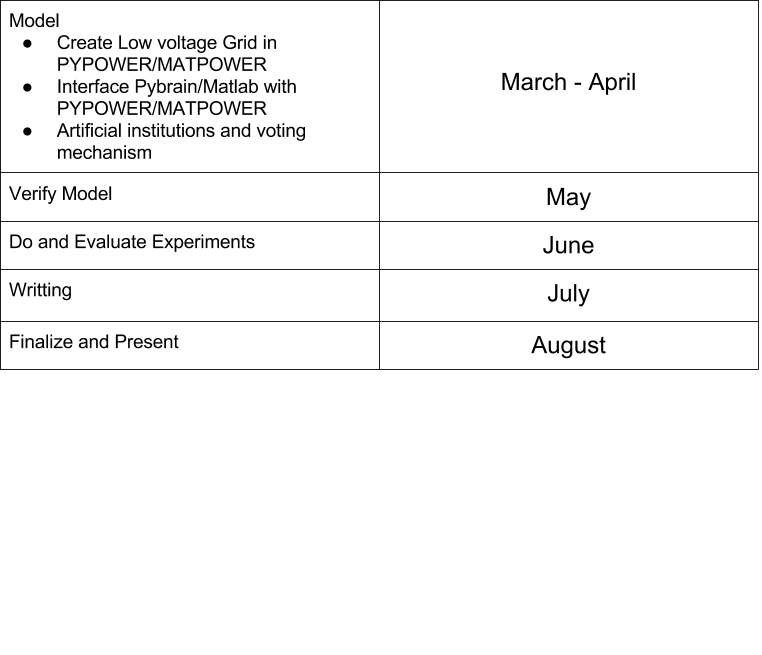
\includegraphics[width =\textwidth]{Time_schedule.png}
\caption{Time Schedule}
\label{time_schedule}
\end{figure}
Besides the general difficulties of doing a master thesis project there are a few pitfalls of this project that are worth mentioning.
\begin{enumerate}
\item Implementation \begin{enumerate}
\item I am not sure how well PYPOWER/MATPOWER is equipped to deal with a low voltage distribution grid. It is surely possible but there is still the question about how much has to changed. If it is merely a problem of changing parameters or if the code has to altered.
\item I am not sure how easy it will be to use PYPOWER/MATPOWER as an environment for Q-learning algorithms
\item Agents might interfere and cause problems. For instance, if all the agents decided independently to reduce their consumption at one point in time, it would cause the gird to relax in the next time step. Then each agent would independently decide that now that the grid is much more relaxed, more power can be drawn again. The agents might then jump between these two states. 
\item Voting mechanism might have to be very simplistic to be feasible
\end{enumerate}
\item Writing\begin{enumerate}
\item When describing the design philosophy it might be that the topic gets out of hand. There are simply to many things that smart grid touch upon to easily cut it down into very specific things to talk about. 
\end{enumerate}
\end{enumerate}

\section{Graduation Committee}
\begin{figure}[!ht]
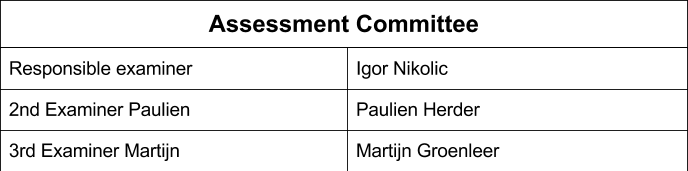
\includegraphics[width =\textwidth]{assessment_committee.png}
\caption{Assessment Committee}
\label{assessment}
\end{figure}
\end{comment}

\newpage

\appendix

\section{PYPOWER Model}
To have some grid to work with a low voltage case has to be created from the ground up, since MATPOWER/PYPOWER does not include any generic low voltage cases. Since there is no data on a real grid, reasonable values have to be assumed based on literature. To create the model the size and topology of a grid has to be set, impedance values for connections and load values for the buses have to be found and all the data has to be converted to per unit values. \\ 
Based on literature\cite{powerbook} a radial network with a central transformer with a power of between 100 and 500kVA is chosen. There will be 24 homes, base load of 6kVA, connected to the transformer with 4 lines. Between each household there will be a line of 100 meters. This way the total base load is about $S_{base}=144kVA$ and the total length of each cable is 600 meters. The base voltage of the grid is 400V. \\
\begin{equation}
Z_{base}=\frac{V_{Base}^2}{S_{Base}}=\frac{(400V)^2}{144kVA} = 1.11\frac{V}{A}
\end{equation}
The low voltage cables are taken from real world cable data and have the following values\cite{cabletable}. 
\begin{enumerate}
\item A= 500 $mm^2$
\item l = 100m = 0.1km
\item R = 0.1590 $\Omega/km * 0.01km = 0.001590$
\item X = 0.0814 $\Omega/km * 0.01km =  0.000814$
\end{enumerate}
The per unit values for the lines therefor are $r = \frac{R}{Z_{Base}}=0.001431$
and $x=\frac{X}{Z_{Base}}=0.00073226$
\begin{figure}[!ht]
\centering
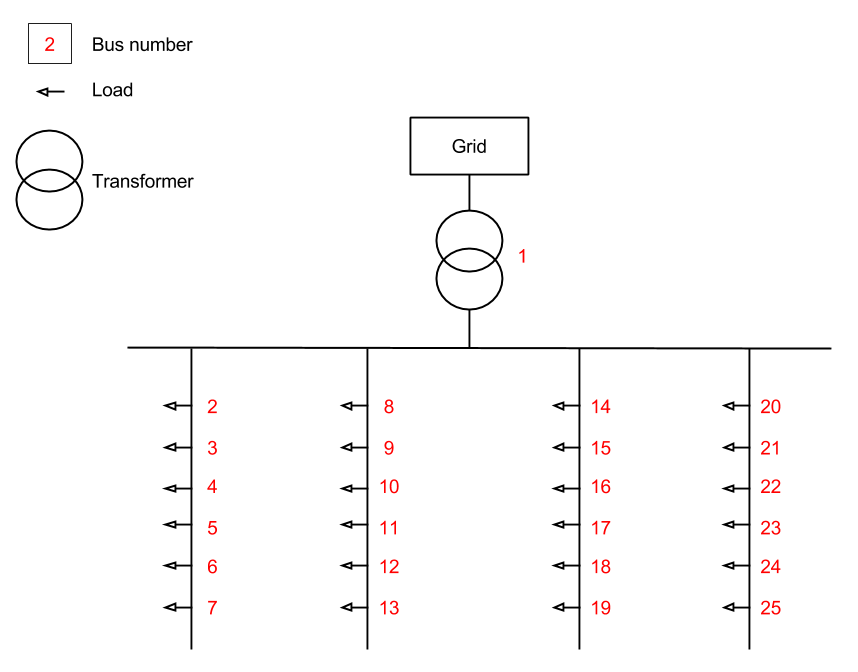
\includegraphics[width = \textwidth]{Topology.png}
\caption{Topology}
\label{topology}
\end{figure}
The load profiles are based on normalized profiles with an  average usage of 8000kWh a year, see figure \ref{profile}. \\
\begin{figure}
\centering
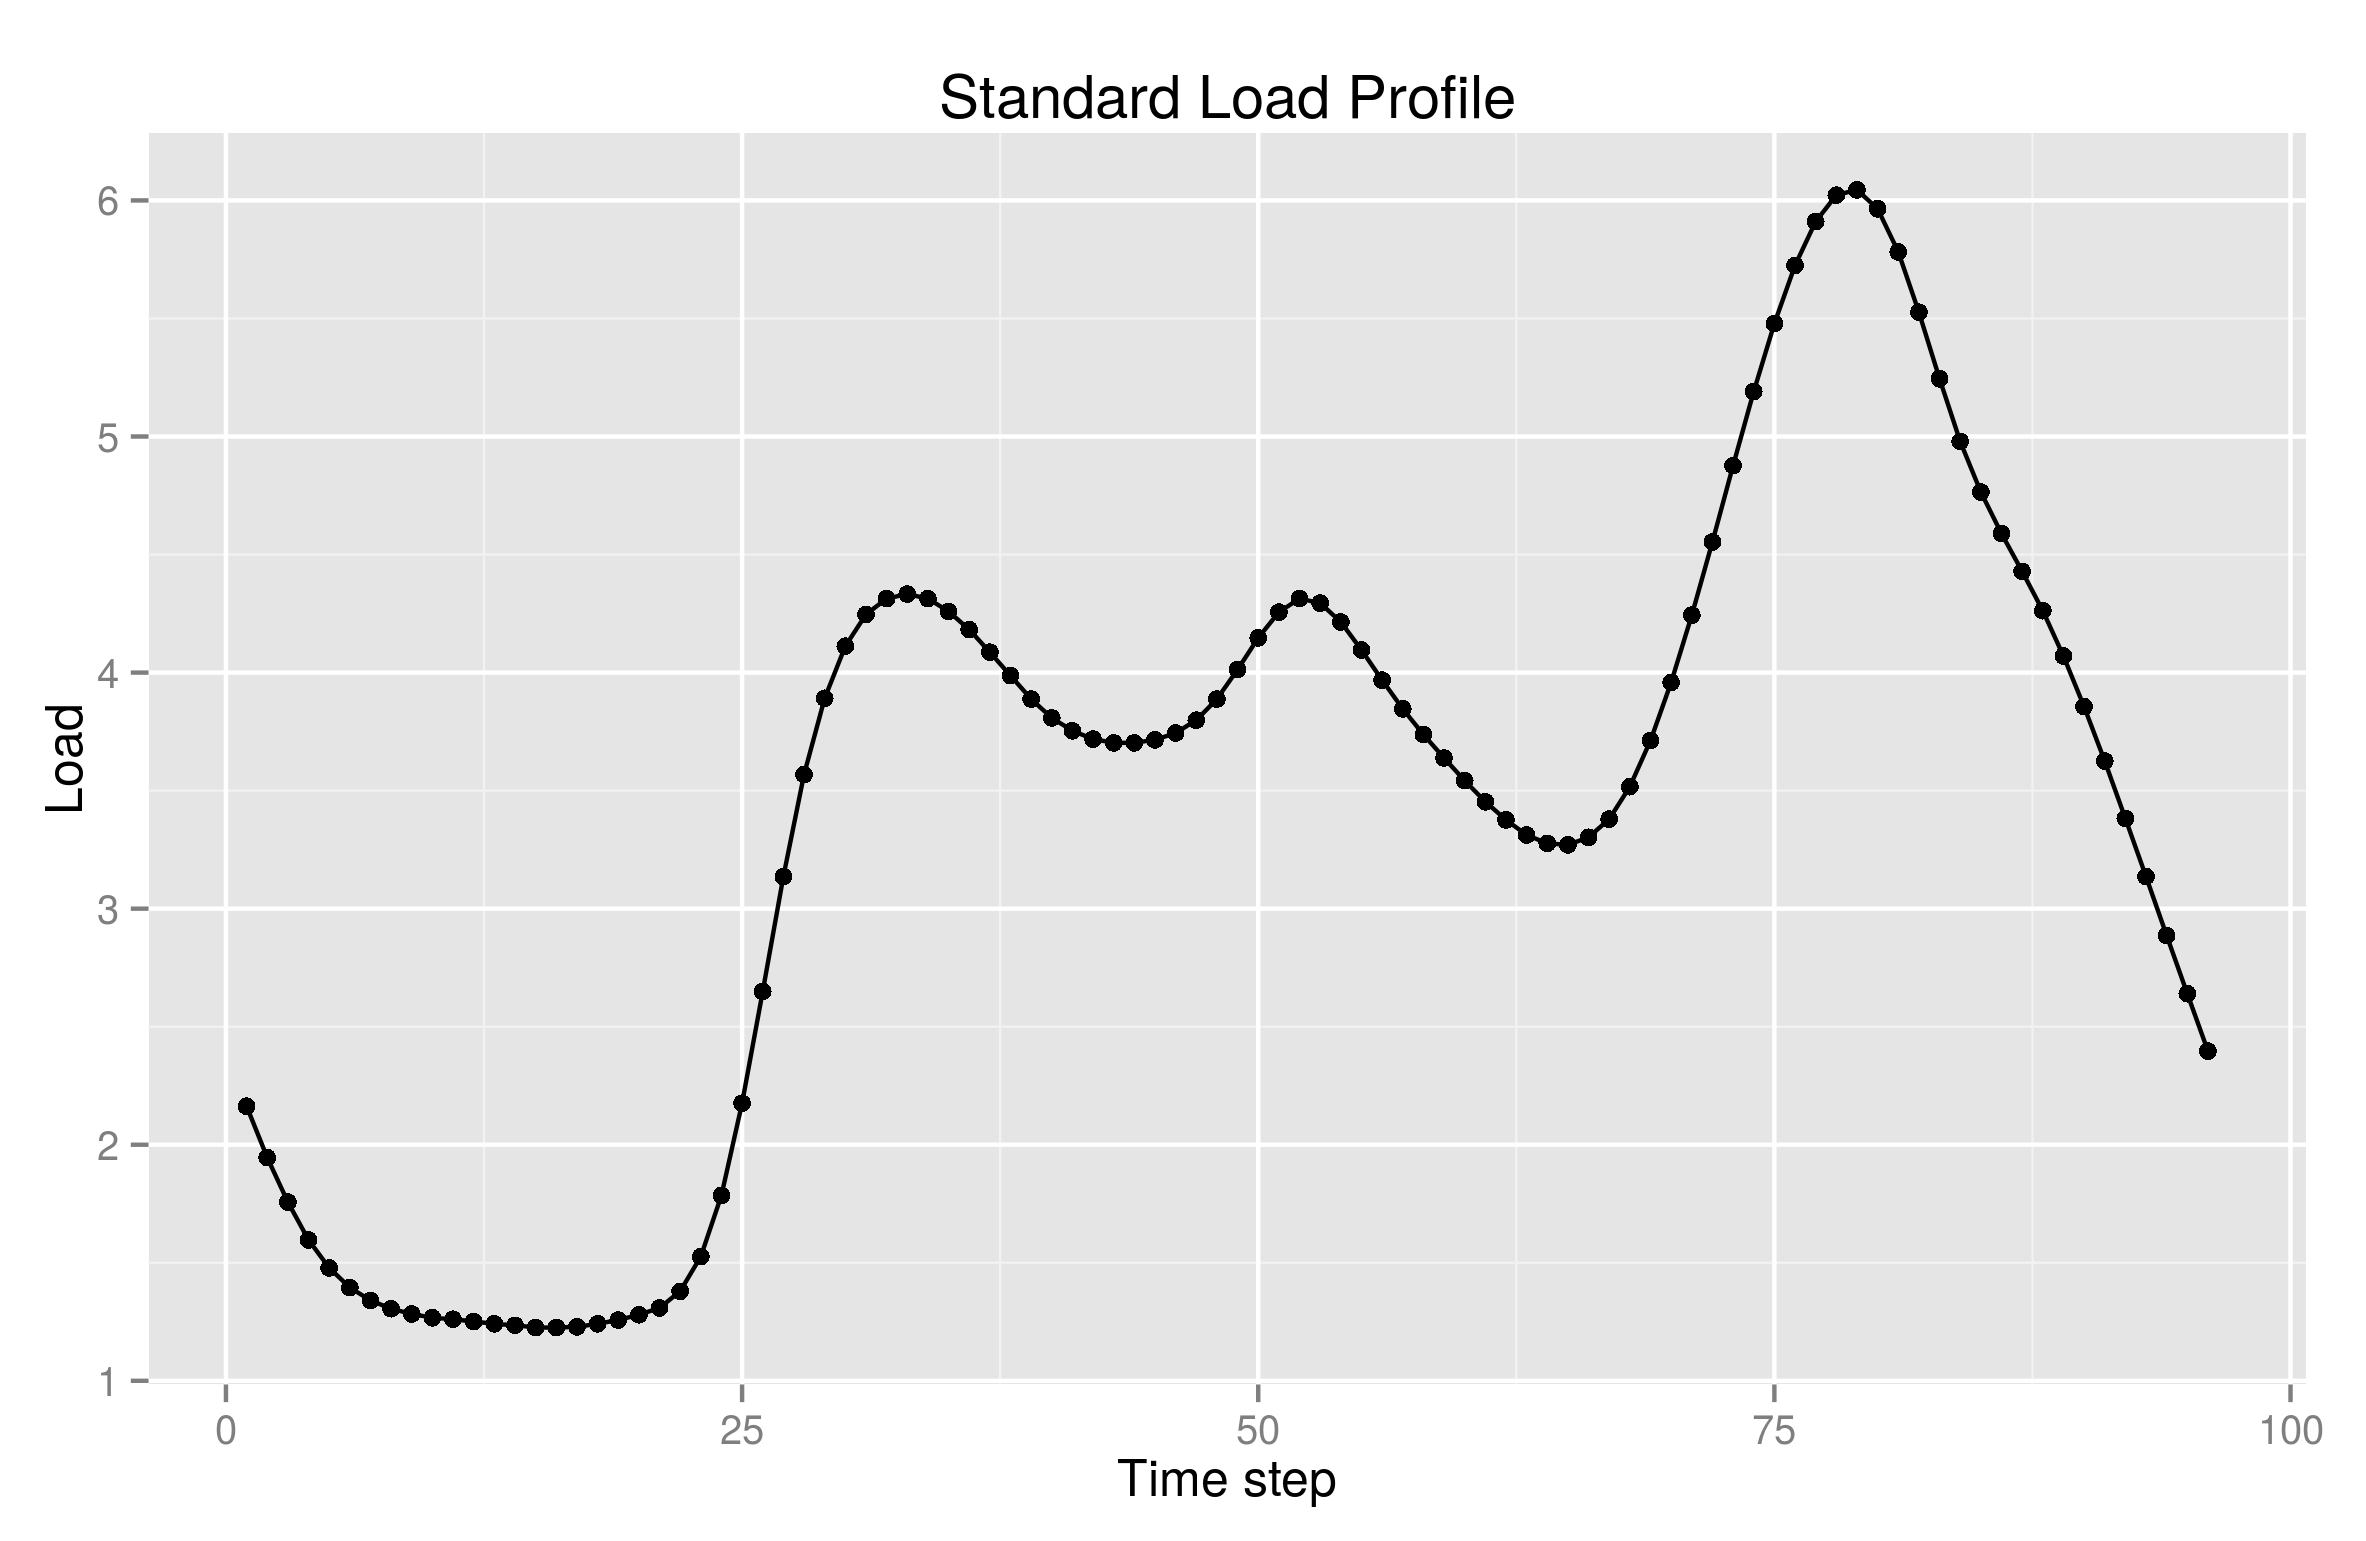
\includegraphics[width = \textwidth]{loadprofile.png}
\caption{Load Profile}
\label{profile}
\end{figure}

\clearpage
\section{Verification}
The verification of the model is done in three steps. The functions that the agent can execute by itself
are verified, then the functions that only work by interacting with other agents or other parts of the
model are verified and finally the pypower model, in particular the constraints. 
\subsection{Verification of Functions}
Each function and how it was tested will shortly be explained. 
\subsubsection{Verification of simple functions}
\begin{enumerate}
 \item \begin{alltt}\textbf{Init_simple_test:}\end{alltt}
  Simple test if an initialized agent is set to the correct state of charge and time.
  
  \item \begin{alltt}\textbf{update_situation:}\end{alltt}
  \textit{Updates the count values and sets a new preference value.}\\
  Agent was initialized with a specific state of charge. State of charge was reset to different values and
  update situation was called every time. The preference value was calculated by hand and compared to 
  the preference value the agent held
  
  \item \begin{alltt}\textbf{Reset_values:}\end{alltt} 
  \textit{Resets the count values (count\_steps,count\_soc,preference) to 0.} \\
  Agent was initialized  and updated the state of charge was then updated several times and 
  the reset values function was called and the count values were checked to be 0.
  
  \item \begin{alltt}\textbf{power_used:}\end{alltt} 
  \textit{Receives an amount of power and updates the state of charge of the battery accordingly.}\\
  Agent was initialized  with a specific state of charge, power used was called and the new state of charge 
  of the agent was compared to the state of charge that was calculated by hand. Agent was also initialized 
  to a state of charge close to full charge, power used was called and it was checked if the state of charge
  would be bound to the maximum soc.
  
  \item \begin{alltt}\textbf{get_action:}\end{alltt}
  \textit{Returns the action, the agent will take based on the agents state.}\\
  Agent was initialized with specific state (voltage,time and SOC). Agent was given 4 different 
  voltage rules,differing in their voltage and state of charge threshold, resulting in different actions.
  The actions the agent was returning was compared to the action it was supposed to take. The same was done
  with 4 different time based rules.
  
  \item \begin{alltt}\textbf{update_memory:}\end{alltt}
  \textit{Takes the active rule and the preference value and adds it to the memory.}\\
  Agent was initialized and the memory of this agent was set. An active rule, which was new to 
  the memory was set. Two test were made, one where the preference value for the active rule was set 
  in such a way that it was worse than the worst rule in the memory and one where it was better than the 
  worst preference value in the memory. The update memory function was called and it was checked if the new 
  rule was in the correct spot in the memory. Then a active rule was set which was already known to the memory. 
  The update memory rule was called and it was checked if the preference value was reset to the average of the two 
  preference values. 
  
  \item \begin{alltt}\textbf{weighted_time_rules:}\end{alltt}
  \textit{Creates a new time based rule based on the rules and preference values in the memory.}\\
  Agent was initialized.  Memory only consisting of time rules was set and the weighted time rules 
  function was called. A new rule was calculated by hand and compared to the rule that was created by 
  the function. The same procedure was repeated with a mixed memory of time and voltage based rules. 
  
  \item \begin{alltt}\textbf{weighted_voltage_rules:}\end{alltt}
  \textit{Creates a new voltage based rule based on the rules and preferences in the memory.} \\
  Same procedure as the weighted time rules function.(see above) 
  
  \item \begin{alltt}\textbf{Arrive_at_home:}\end{alltt}
  \textit{Changes the at\_home variable to True and discharges the battery.} \\
  Agent was initialized and its at\_home variable was set to False. The arrive at home  
  function was called 
  and the at\_home variable was checked to be True. Further the state of charge was set to “-2” and the 
  arrive at home function was called . The state of charge of the agent was checked to be reset to 0.
\end{enumerate}

\subsubsection{Verification of interacting functions:}
\begin{enumerate}
 \item \begin{alltt}\textbf{copy_best(all):}\end{alltt}
 \textit{Searches through all other agents and copies the rule with the highest preference value.} \\
 24 Agents were initialized and each agent expect one was given the same memory. The one exception
 was give a memory with a rule with a preference value that was higher than the others. The copy best 
 function was called from one of the other agents. The new active rule of this agent was compared to the 
 one rule with the highest preference in the special agent. 
 
 \item \begin{alltt}\textbf{copy_best(vertical):}\end{alltt}
 \textit{Searches through all other agents, in the same branch,  and copies the rule with the highest preference value.}\\
 24 agents were initialized and each agent except for two were given the same memory. The copy\_all 
 variable was set to “vertical”. There is one original agent on which the copy\_best function will then 
 be called on. One exception was in the same branch as the original agent and  given a better rule. 
 The second exception was given a global best rule in its memory and placed outside of the original 
 agents branch. The two exceptions are on the same level but in different branches.  The agent should when
 the copy best function is called on it find the best rule in its branch but ignore the global best rule. 
 
 \item \begin{alltt}\textbf{copy_best(horizontal):}\end{alltt}
 \textit{Searches through all other agents, on the same level,  and copies the rule with the highest preference value.}\\
 24 agents were initialized and each agent except for two were given the same memory. The copy\_all 
 variable was set to “horizontal”.There is one original agent on which the copy\_best function will then 
 be called on. One exception was on the same level as the original agent and  given a better rule. The second
 exception was given a global best rule in its memory and placed outside of the original agents level. The 
 two exceptions are on the same branch but in different levels.  The agent should when the copy best function 
 is called on it find the best rule in its level but ignore the global best rule. 
 
 \item \begin{alltt}\textbf{do_interaction:}\end{alltt}
 \textit{Receives a pypower model as input and adds power to the node of the agent based on the active rule of the agent.}\\
 24 Agents were initialized. Each agent was given a different node but the same voltage, active rule, 
 state of charge and time.  A pypower model was initialized to the same time as the agents. Each agent called 
 the do interaction function on the pypower model. A theoretical load vector was calculated by hand and compared 
 to the load vector in the pypower model after the interaction with the agents. 
 
 \item \begin{alltt}\textbf{get_feedback:}\end{alltt}
 \textit{Receives a pypower output structure as input and updates the state of charge of the battery 
 based on how much power was actually used.} \\
 24 Agents were initialized. The 24 Agents were given the same state and the same active rule. 
 A pypower  model was initialized and its voltage constraints were removed to make the amount of power 
 used predictable. Each agent was interacting with the pypower model and the get feedback function 
 was called for each agent. A new state of charge was calculated by hand and compared to the new state of
 charge of the agents after the function call.
 
 \item \begin{alltt}\textbf{Voting:}\end{alltt}
 \textit{Takes the memory of all the agents, combines them into an election matrix ,taking 
 the individual memory matrices as borda count votes. }\\
 24 Agents were initialized, each agent was given the same memory. Then the voting algorithm was called.  
 The number each rule should be represented in the election matrix was calculated by hand and compared to 
 the actual number of occurrences in the election matrix. Further the total number of voltage rules and the 
 total number of time rules was calculated by hand and compared to the actual number of time and voltage rules 
 in the election matrix. The k-means clustering algorithm was not tested since it is a function of the numpy python package.
\end{enumerate}

\subsection{Verification of Pypower model}
The functions that are to be verified are the following. 
\begin{enumerate}
 \item The dispatchable loads are \begin{enumerate}
                                   \item changed in such a way that  the voltage at each node is 
                                   always above a specific voltage threshold
                                   \item not changed if the voltage is already above the specific voltage threshold
                                   \item changed first at the nodes with the highest voltage in the branch
                                  \end{enumerate}

\end{enumerate}
To verify this two pypower models are initialized one with and  one without a voltage constraint. Both models are 
run 20 times. Each time a random dispatchable load is applied to the different node points. Within each run the 
dispatchable loads of both models are set to the same values. Among other things the voltage is kept track of and compared. 
The two graphs below show the minimum voltage in each branch. The red line indicates the voltage threshold.  In the
top graph the unrestricted load causes the voltage to drop below the voltage threshold, in the bottom graph 
the minimum voltage seems to be bound to the red line while the points above the line appear to be unchanged. 
This is confirmed by looking at the dispatchable load in the branches which had a minimum voltage above the threshold
in the unconstrained case. In those cases the dispatchable loads of both models were exactly equal. To check if the order
in which the loads are cut is correct, the percentage of change between the constrained and unconstrained case is checked
for each branch. If  at any node the change is more than 0 and below 100 percent, this node has to be either the very 
lowest in its branch , meaning furthest away from the source and therefore lowest voltage, or all the percentage difference 
that come after it in the branch have to be 100 percent. 
All the test are run in the “pypower\_constraint\_test.py” file. 


\begin{figure}[!ht]
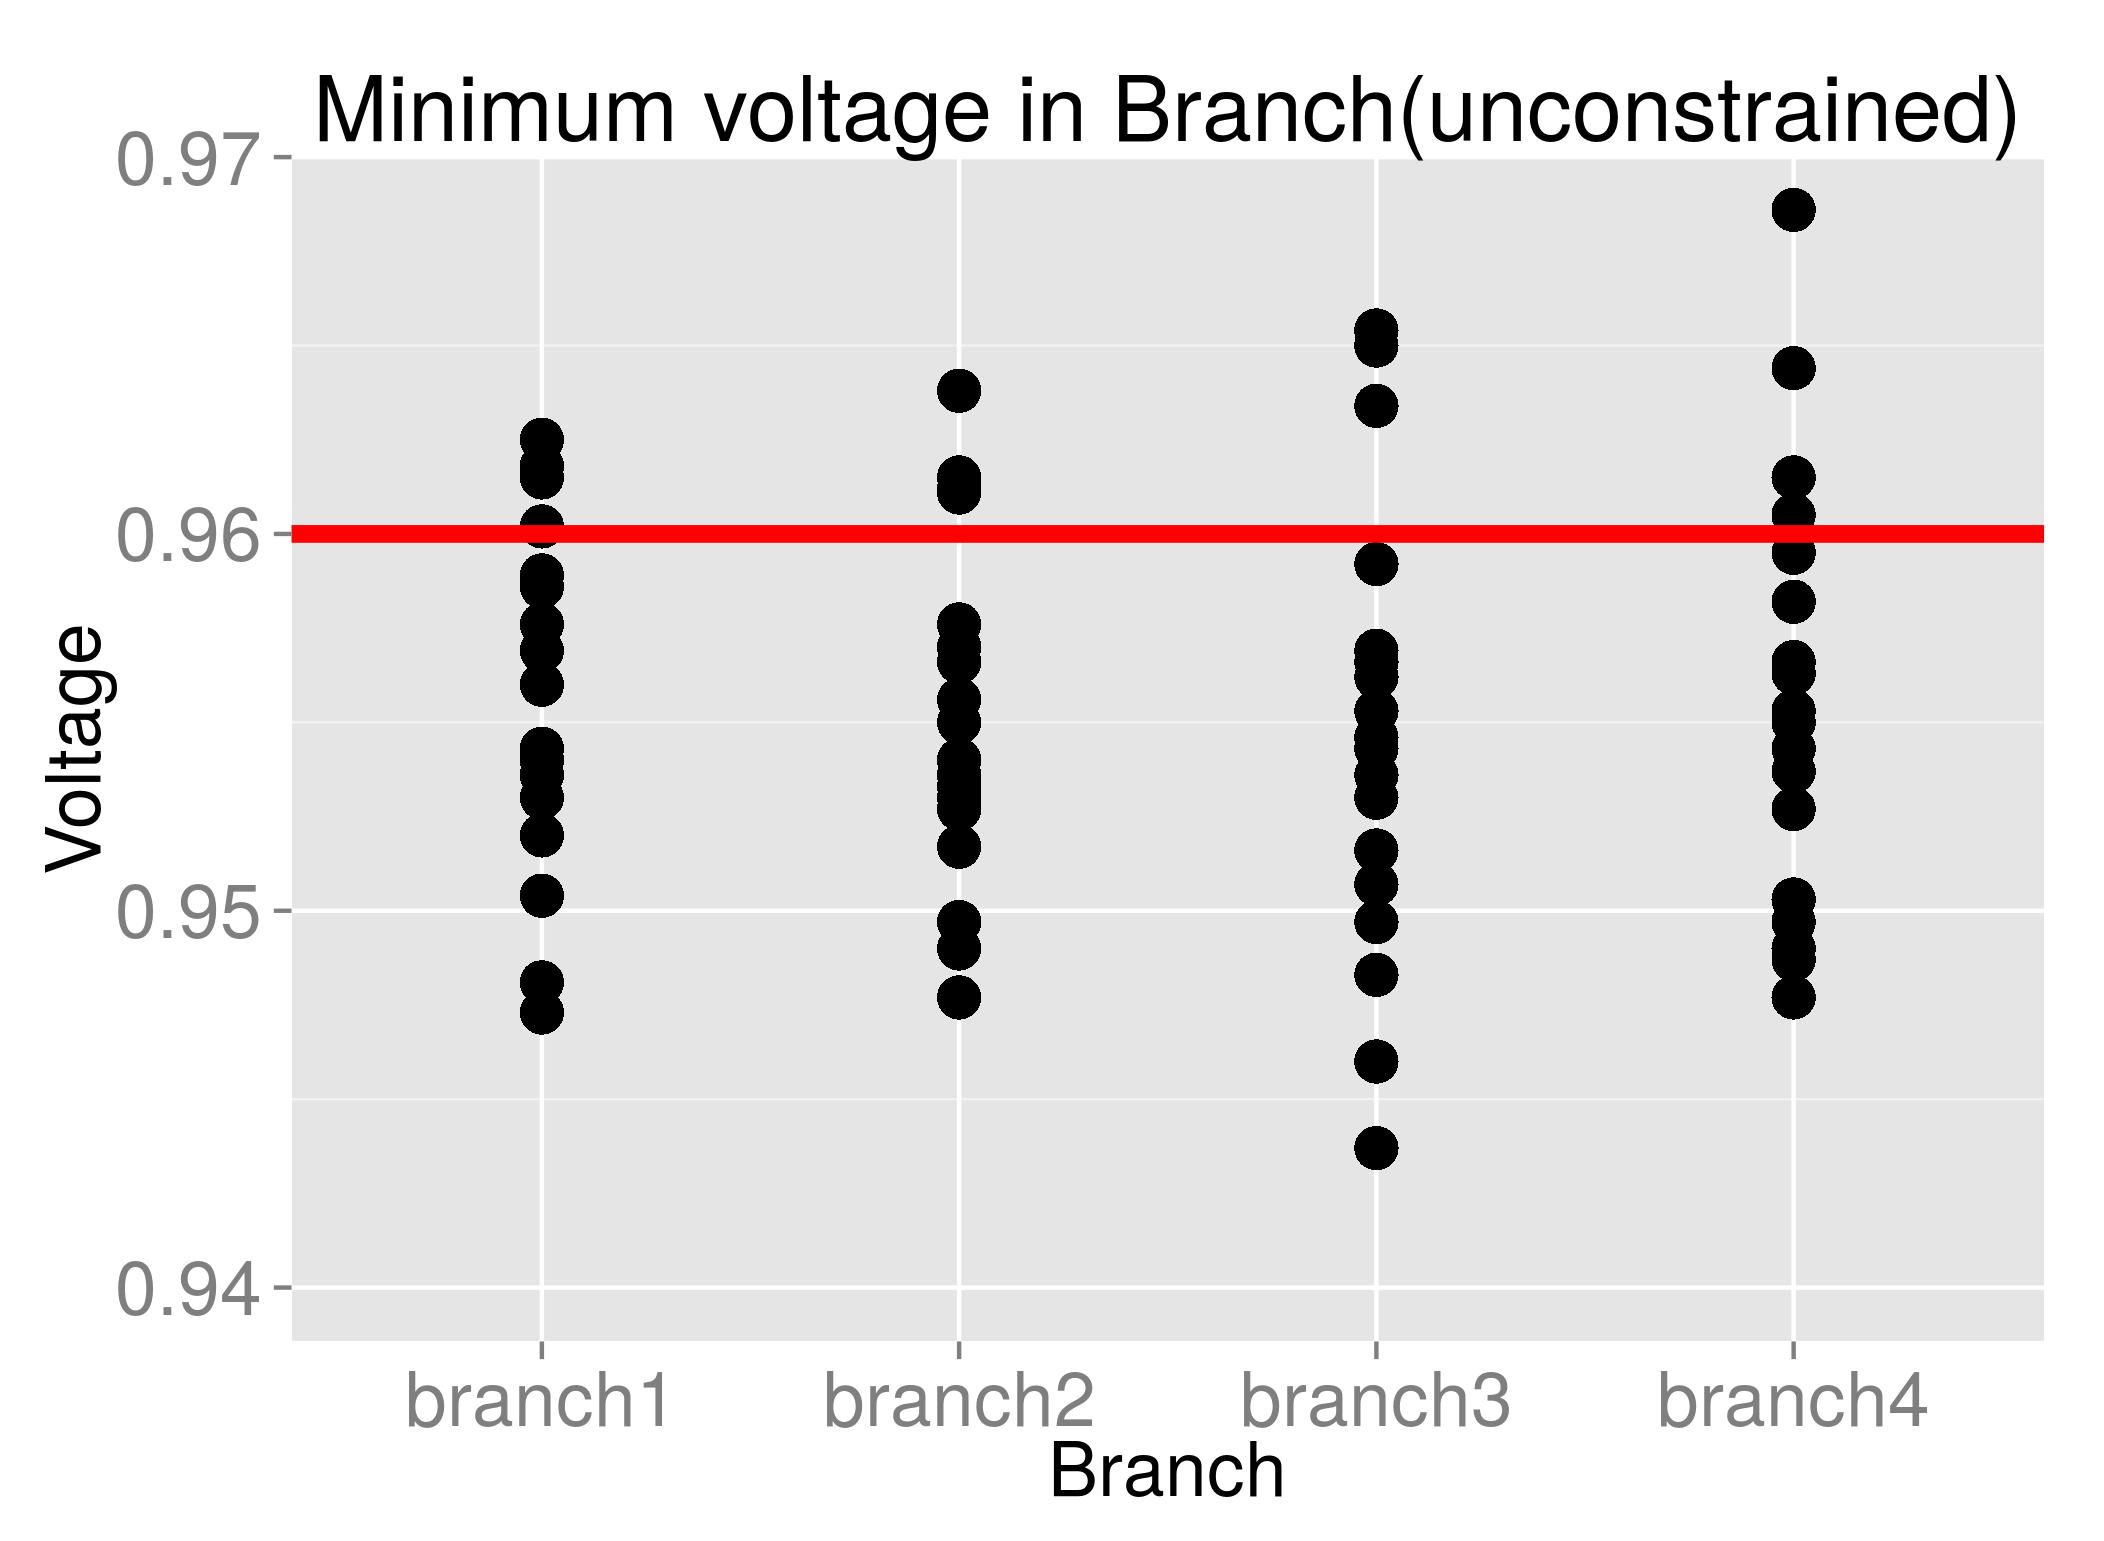
\includegraphics[width =\textwidth]{unconstrained.jpg}
\caption{Pypower model without constraints}
\label{un_constrained_pypower}
\end{figure}

\begin{figure}[!ht]
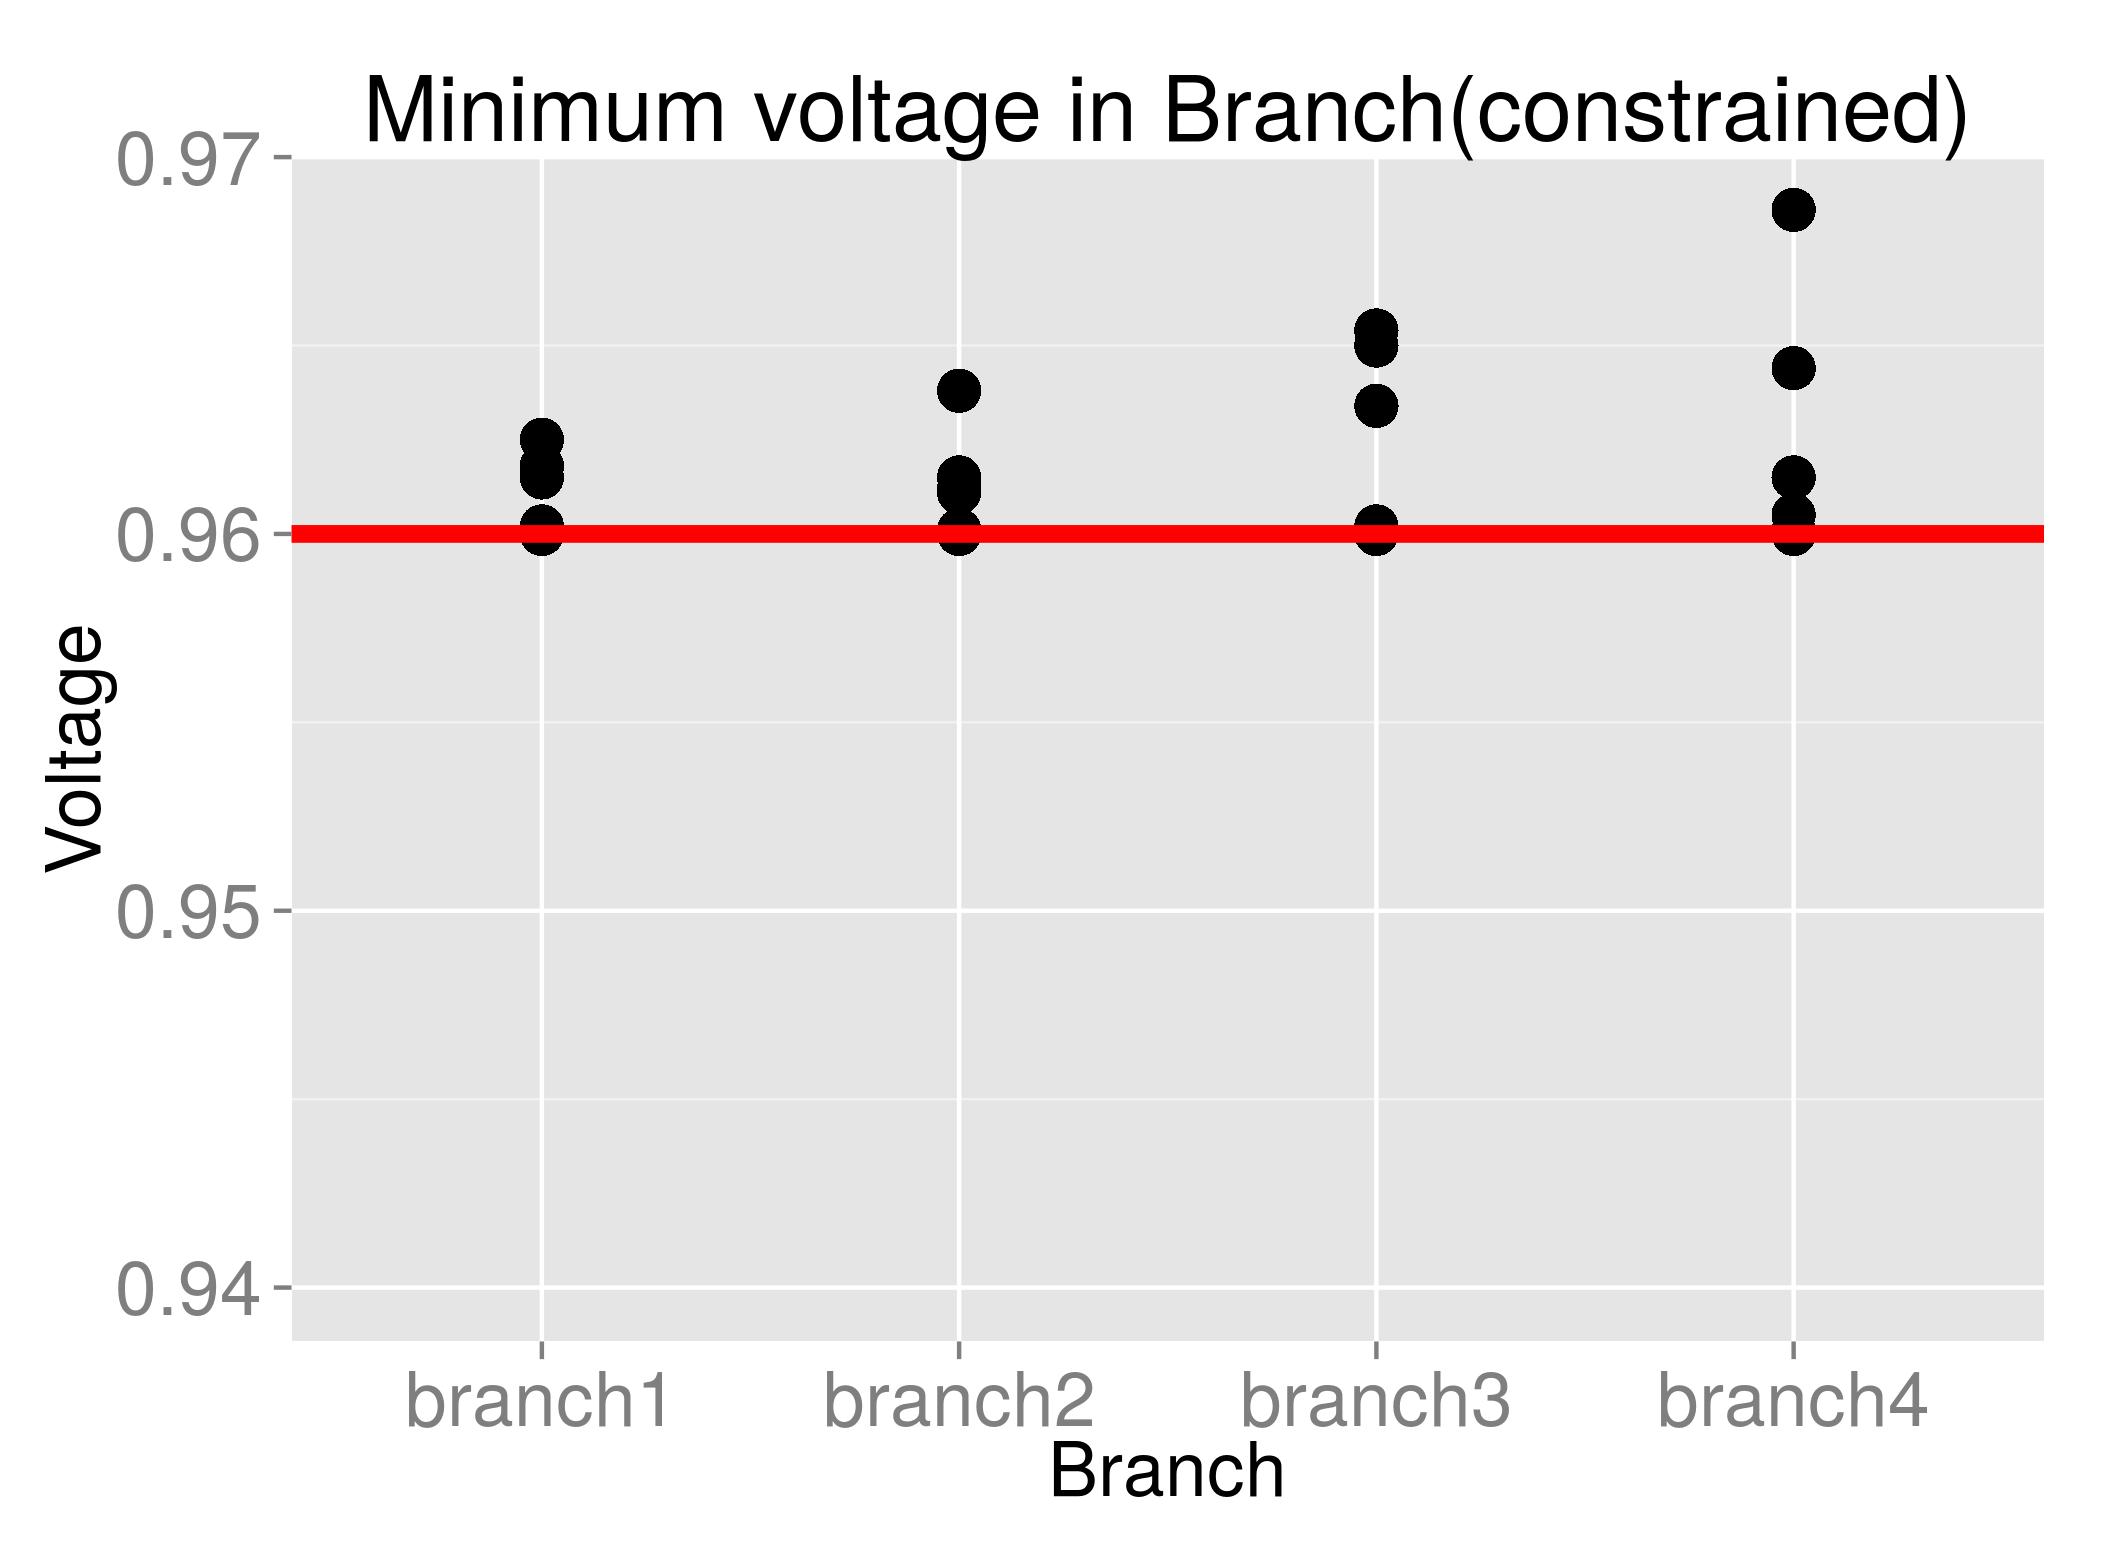
\includegraphics[width =\textwidth]{constrained.jpg}
\caption{Pypower model with constraints}
\label{constrained_pypower}
\end{figure}
\newpage
\section{Pseudo Code}
\begin{enumerate}
 \item Agents have:\begin{enumerate}
                    \item active\_rule
                    \item Memory (7,5 Matrix)
                    \item arrival\_time
                    \item leaving\_time
                    \item at\_home (true/false)
                    \item average\_battery\_drain
                    \item sd\_battery\_drain
                    \item SOC
                    \item SOC\_max
                    \item Voltage
                    \item Node
                    \item count\_steps
                    \item count\_soc
                    \item preference
                    \item copy\_all
                   \end{enumerate}
 \item Global Variables: \begin{enumerate}
                          \item average\_arrival\_time
                          \item average\_leaving\_time
                          \item sd\_average
                          \item average\_battery\_drain
                          \item sd\_average\_battery\_drain
                          \item average\_soc
                          \item sd\_average\_soc
                          \item soc\_max\_global
                          \item random\_change
                          \item copy\_best\_change
                          \item learn\_change
                          \item Action\_options
                          \item t\_end\_options
                          \item t\_begin\_options
                          \item soc\_threshold\_options
                          \item voltage\_options
                          \item institutional\_rule
                          \item institutional\_success\_rate
                         \end{enumerate}
\end{enumerate}

\newpage
In the setup phase of the model the time gets set to 0, the agents are created and initialized and the 
matpower model is created. 

\begin{figure}[!ht]
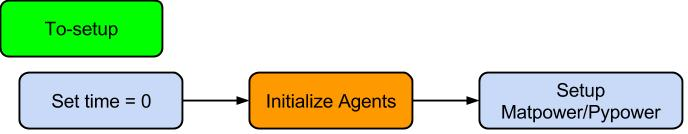
\includegraphics[width =\textwidth ]{setup.jpg}
\caption{To-setup}
\label{setup}
\end{figure}
During the initialization the agents get assigned their node in the grid and the voltage is set to 
1. Each agent then initializes their preference to the current rule to 0, sets leaving and arrival times, 
sets up their battery and creates an initial rule and an empty Memory.
\begin{figure}[!ht]
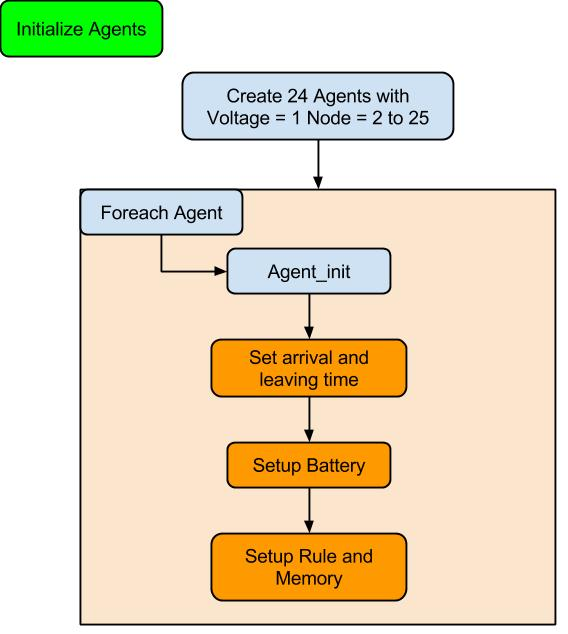
\includegraphics[width = 10cm]{init_agent.jpg}
\caption{Initialize agents}
\label{init_agents}
\end{figure}
\begin{alltt}
 \underline{\textit{Pseudo Code:}}
create-turtles agents 24 [set voltage to 1 set node to 2-25]
Foreach Agent
    set count_steps = 0 
    set count_soc = 0 
    set preference = 0
    Set arrival and leaving time
    Setup Battery
    Setup Rule and Memory
\end{alltt}

\begin{figure}[!ht]
\centering
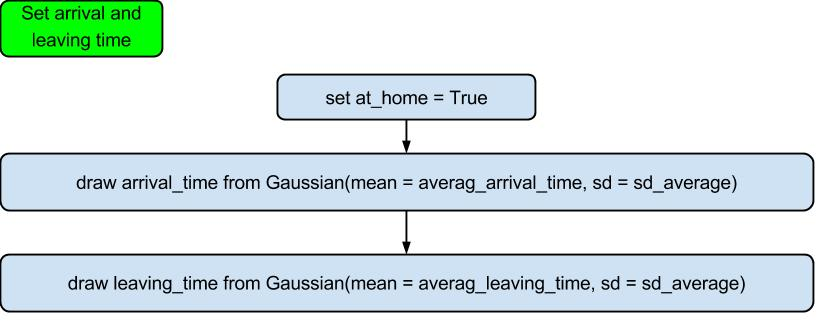
\includegraphics[width =10cm]{set_arrival_leaving_time.jpg}
\caption{Setup arrival and leaving time}
\label{setup_arival_leaving}
\end{figure}


\begin{figure}[!ht]
\centering
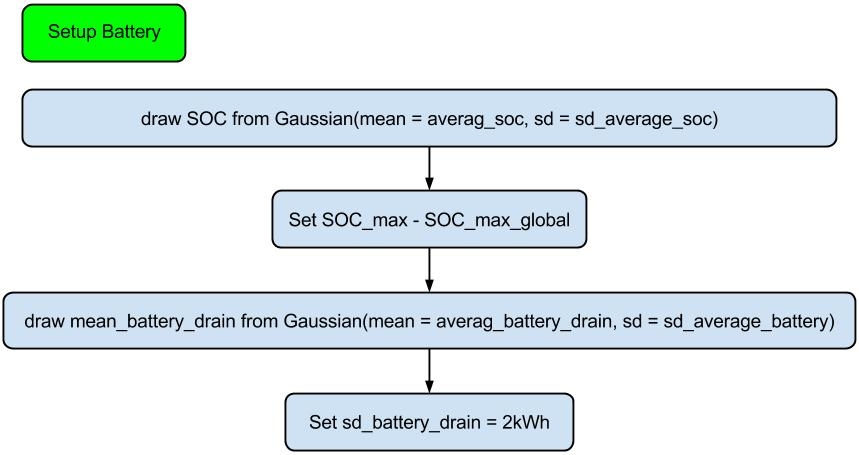
\includegraphics[width =10cm]{setup_battery.jpg}
\caption{Setup Battery}
\label{setup_battery}
\end{figure}

\begin{figure}[!ht]
\centering
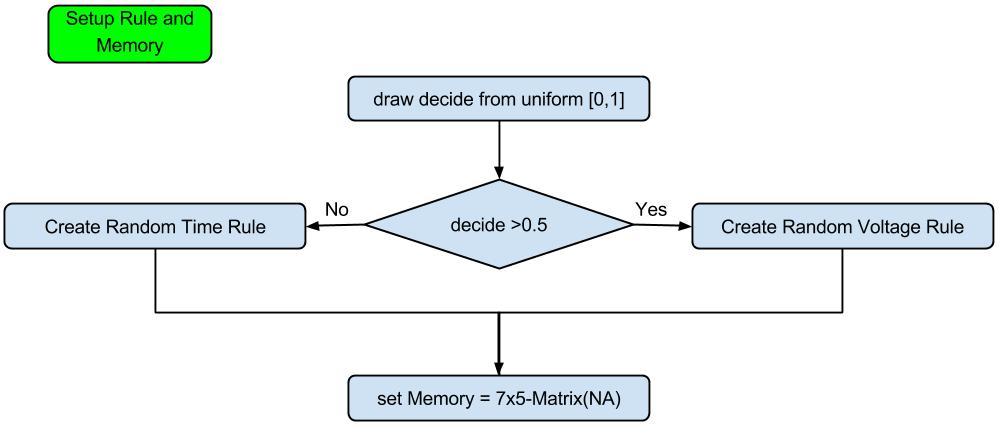
\includegraphics[width =10cm]{setup_rule_memory.jpg}
\caption{Setup Rules and Memory}
\label{setup_rule_memory}
\end{figure}

\begin{alltt}
 \underline{\textit{Pseudo Code:}}
let decide be a random number between 0 and 1
if decide > 0.5 
    let t\_begin be randomly picked from t_begin_options
    let t\_end be randomly picked from t_end_options
    let soc\_threshold be randomly picked from soc\_threshold_options
    let action1 be randomly picked from action\_options
    let action2 be randomly picked from action\_options
    set active\_rule to vector[2,t\_begin,t\_end,soc\_threshold,action1,action2]
else
    let voltage_threshold be randomly picked from voltage_threshold_options
    let soc_threshold be randomly picked from soc_threshold_options
    let action1 be randomly picked from action_options
    let action2 be randomly picked from action_options
    set active_rule to vector[1,voltage_threshold,soc_threshold,action1,action2,NA]

let Memory be a 7X5 matrix of NA values
\end{alltt}
\newpage

To-go \\
The two things the agents do in the to-go part is to interact with the matpower model and develop rules.
\begin{figure}[!ht]
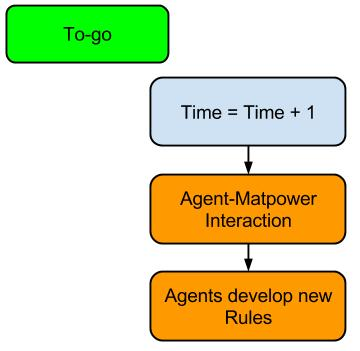
\includegraphics[width =\textwidth]{go.jpg}
\caption{To-go}
\label{to-go}
\end{figure}
The agents interact with the matpower model by inputting their action into the matpower model,
the model then runs and outputs a structured output object. From this output object the agents read
the actual power they received. The agents can only interact with the model if they are at home. 
The agents arrive and leave at specific times, and this state is kept track of by the at\_home variable.
\newpage
\begin{figure}[!ht]
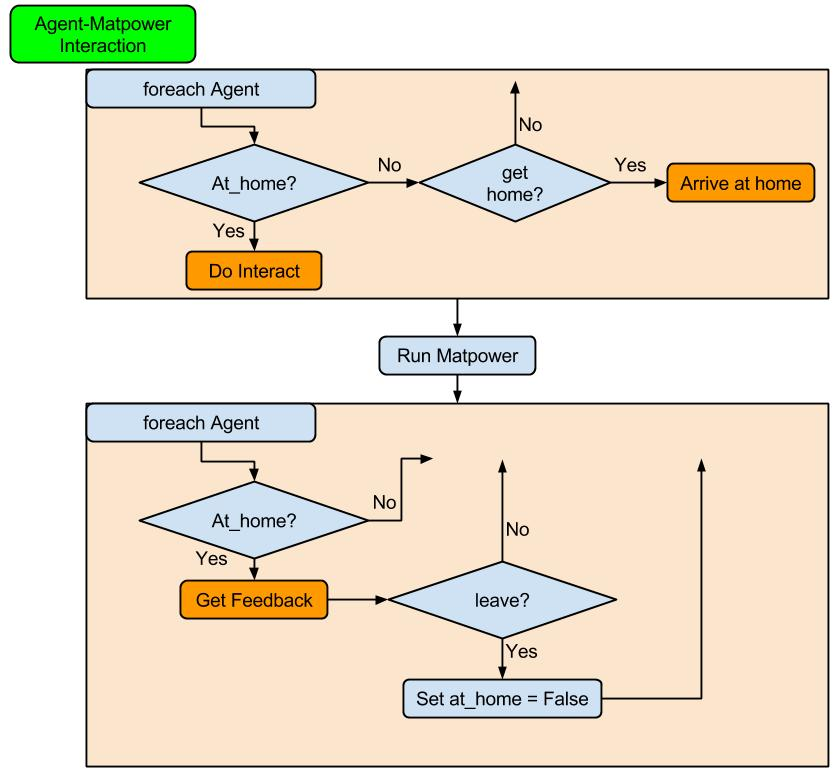
\includegraphics[width =\textwidth]{agent_matpower_interaction.jpg}
\caption{Agent matpower interaction}
\label{agent-matpower-interaction}
\end{figure}
\begin{alltt}
 \underline{\textit{Pseudo code:}}
foreach agent
    if (at_home ==True)
        Do Interact
    else 
        if (time%96 == arrival_time)
            Arrive at home
Run Matpower
foreach agent
    if (at_home == True)
        get feedback 
        if (time % 96 == leaving_time)
            set at_home to False
\end{alltt}
\newpage
\begin{figure}[!ht]
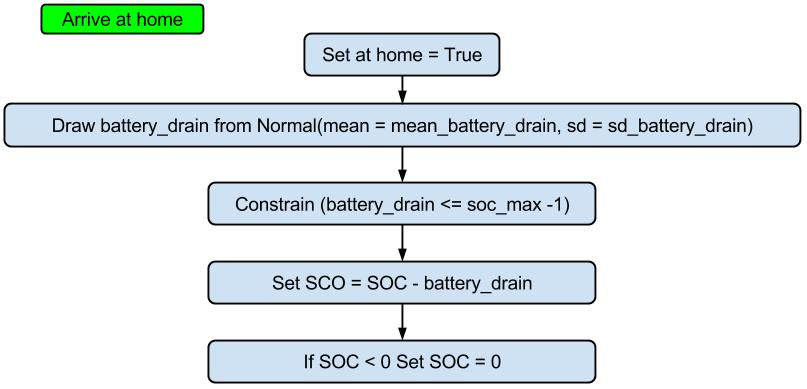
\includegraphics[width =\textwidth]{arrive_home.jpg}
\caption{Arrive at home}
\label{arrive_at_home}
\end{figure}

\begin{figure}[!ht]
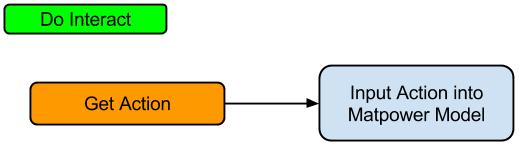
\includegraphics[width =\textwidth]{do_interaction.jpg}
\caption{Do Interact}
\label{do_interact}
\end{figure}

\begin{figure}[!ht]
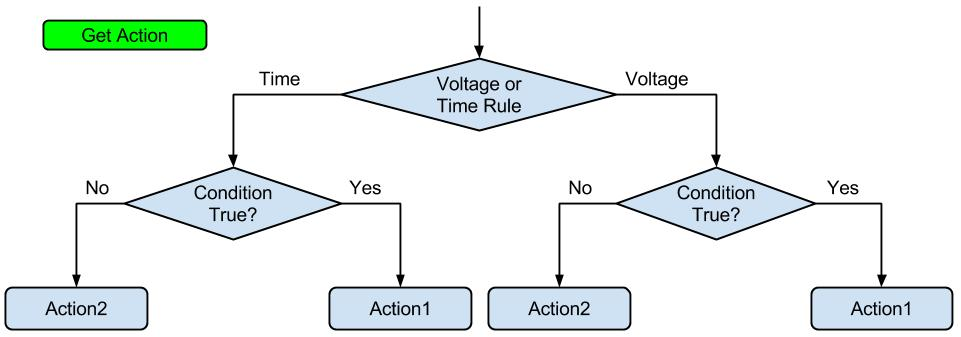
\includegraphics[width =\textwidth]{get_action.jpg}
\caption{Get Action}
\label{get_action}
\end{figure}

\begin{alltt}
 \underline{\textit{Pseudo Code:}}
if (active_rule[index = 1] ==1)
    if (Voltage < active_rule[index = 2]) 
	& (soc > active_rule[index = 1])
        return active_rule[index = 4]
    else 
        return active_rule[index = 5]
else 
    if (active_rule[index = 3] > active_rule[index=2])
        if (active_rule[index = 2] < time\%96 < active_rule[index = 3]
	    &  soc > soc_thres.)
            return active_rule[index = 5]
        else 
            return active_rule[index = 6]
    else 
        if  (active_rule[index = 2] < time\%96  
	      or time  96 < active_rule[index = 3]
	      &  soc > soc_threshold)
            return active_rule[index = 5]
        else 
            return active_rule[index = 6]
\end{alltt}

\begin{figure}[!ht]
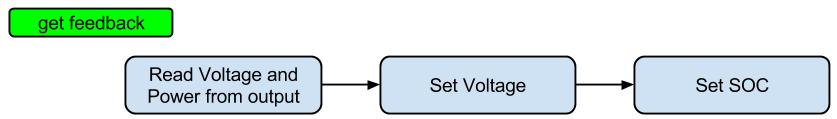
\includegraphics[width =\textwidth]{get_feedback.jpg}
\caption{Get feedback}
\label{get_feedback}
\end{figure}
\begin{alltt}
 \underline{\textit{Pseudo Code:}}
let power be  - 1000.0 * output["gen"][node,1] ;; -1000 stems from unit conversions
let volt be output["bus"][node,7]
set voltage = volt
set SOC = SOC + power/4
if SOC > SOC_max 
    set SOC to SOC_max
\end{alltt}
\newpage

\begin{figure}[!ht]
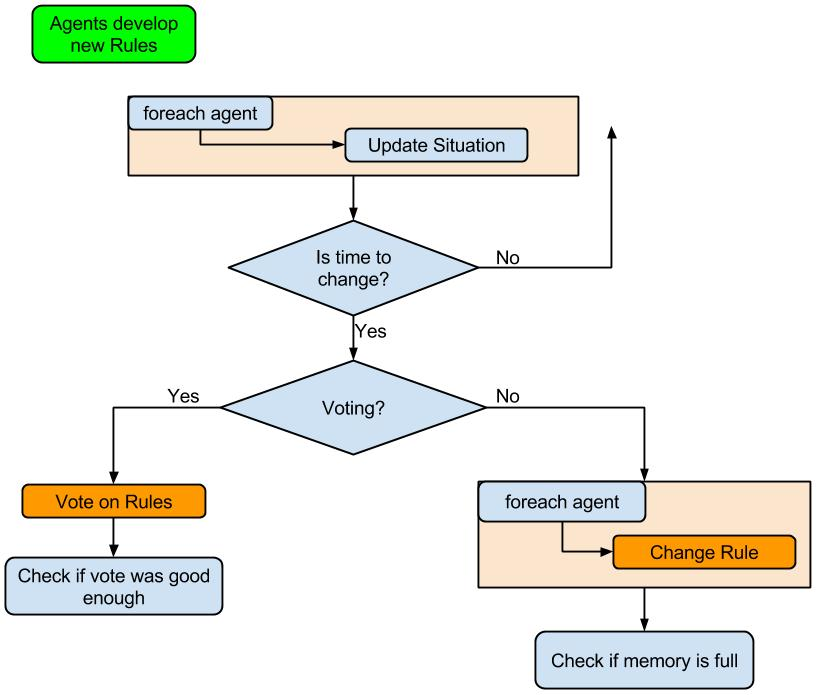
\includegraphics[width =\textwidth]{agents_develop_rules.jpg}
\caption{Agents develop new rules}
\label{agents_develop_rules}
\end{figure}
\begin{alltt}
 \underline{\textit{Pseudo Code:}}
foreach agent
    count_steps = count_steps + 1
    count_soc = count_soc + soc
    preference = count_soc / count _steps ;; basically the average soc 
voting = False
if (time % 672 == 0)                 ;; 672 is one week in 15 minutes ticks
    if (voting == True)             
        if (there is already an institutional rule)
            let counter be the number of times the institutional rule is in agent memory
            if (counter < 24 * institutional_success_rate)
                set voting to False
            Vote on rules
else 
            Vote on Rules

    else 
        foreach agent
            Change Rule
        let in_memory be  True
foreach agent
            if memory is not full 
                set in_memory to False
        if (in_memory == True)
            set voting to True
\end{alltt}

\begin{figure}[!ht]
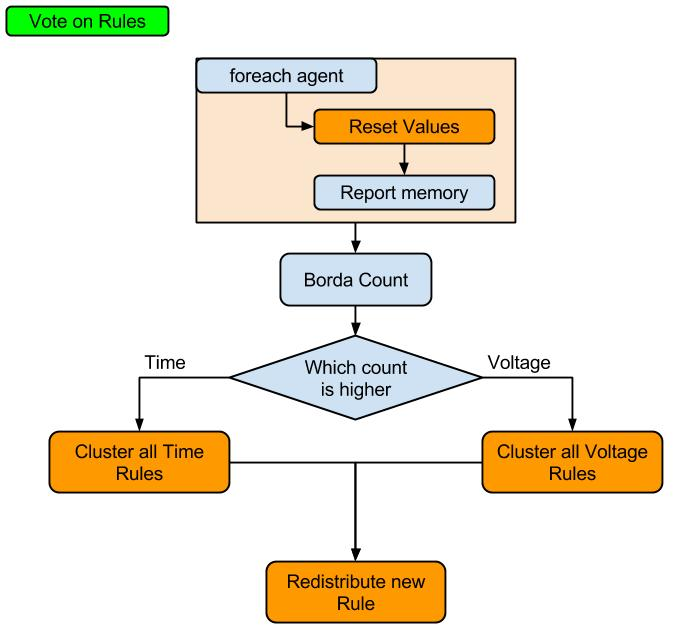
\includegraphics[width =\textwidth]{vote_rules.jpg}
\caption{Vote on Rules}
\label{vote_rules}
\end{figure}
\begin{alltt}
 \underline{\textit{Pseudo Code:}}
let election_list be an empty list of matrices
Foreach agent
    reset Values 
    add Memory to election_list
let election_matrix be a 240x7 empty  matrix
let n be 5  ;; number of rules for borda count
let i be 1 
foreach element in election_list 
    for k = 1 to 5
        let multiple be 0
        while multiple < n-k 
            set election_matrix[index = all, index = i] to element[k, all]
set i to i + 1 
set multiple to multiple + 1 
let number_voltage_rules to number of instances (election_matrix[index = 1, index = all]== 1)
let number_time_rules to number of instances (election_matrix[index = 1, index = all]== 2)
if number_time_rules > number_voltage_rules 
    set new_rule to Cluster all Time Rules
else 
    set new_rule Cluster all Voltage Rules
foreach agent
    set active_rule to new_rule
\end{alltt}

\begin{figure}[!ht]
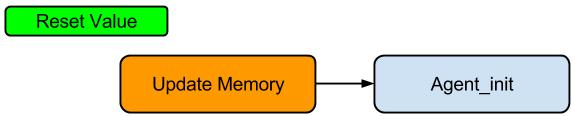
\includegraphics[width =\textwidth]{reset_value.jpg}
\caption{Reset values}
\label{reset_values}
\end{figure}
\begin{alltt}
 \underline{\textit{Pseudo Code:}}
Update Memory 
set count_steps to 0
set count_soc to 0 
set preference to 0 
\end{alltt}

\begin{figure}[!ht]
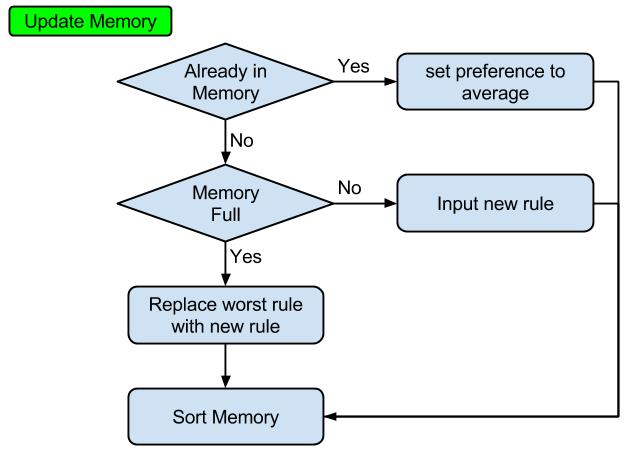
\includegraphics[width =\textwidth]{update_memory.jpg}
\caption{Update Memory}
\label{update_memory}
\end{figure}
\begin{alltt}
 \underline{\textit{Pseudo Code:}}
 let in_memory be False
for k = 1 to 5
    if memory[k ,index 1 to 6] == active_rule
        set in_memory to True
        let memory_index  be k
if (in_memory == True)
    set memory[memory_index,7] = (memory[memory_index,7] +preference)  / 2
else 
    let memory_full be True
    for k = 1 to 5 
        if (memory[k ,1] ==NA) 
            set memory_full to False
            set memory_index to k 
    if (memory_full == True)
        if (active_rule[index = 7] > memory[index = 5m index = ])
            set memory[index = 5, index = 1 to 6] to active_rule
            set memory[index = 5, index = 7] to preference
    else 
        set memory[index = memory_index,index = all] to active_rule
        set memory[index = memory_index, index = 7] to preference
sort memory by 7th column
\end{alltt}

\begin{figure}[!ht]
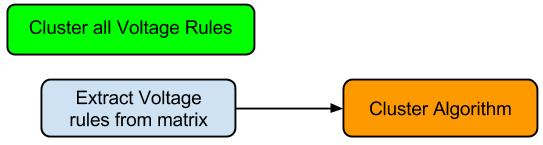
\includegraphics[width =\textwidth]{Cluster_voltage.jpg}
\caption{Cluster Voltage Rules}
\label{cluster_voltage}
\end{figure}
\begin{alltt}
 \underline{\textit{Pseudo Code:}}
let cluster_matrix be a (number_voltage_rules)x7 matrix 
let i be 1
for elements in election_matrix
    if (element[index = 1] == 1)
        set cluster_matrix[index = all, index = i] = element
        i = i + 1
Cluster Algorithm(cluster_matrix)
\end{alltt}
\newpage
\begin{figure}[!ht]
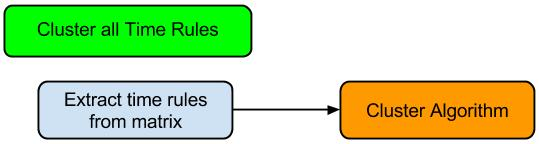
\includegraphics[width =\textwidth]{cluster_time.jpg}
\caption{Cluster time Rules}
\label{cluster_time}
\end{figure}

\begin{alltt}
 \underline{\textit{Pseudo Code:}}
let cluster_matrix be a (number_time_rules)x7 matrix 
let i be 1
for elements in election_matrix
    if (element[index = 1] == 2)
        set cluster_matrix[index = all, index = i] = element
        i = i + 1
Cluster Algorithm(cluster_matrix)
\end{alltt}


\begin{figure}[!ht]
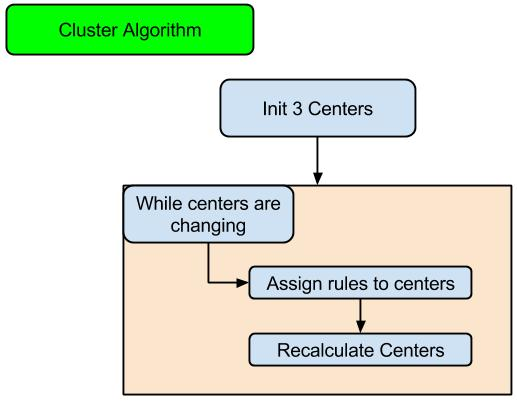
\includegraphics[width =\textwidth]{cluster_algorithm.jpg}
\caption{Cluster algorithm}
\label{cluster_algorithm}
\end{figure}

\begin{alltt}
 \underline{\textit{Pseudo Code:}}
let centers be a 3x6 matrtix
if (cluster_matrix[index = 1, index =1] ==1)
for k = 1 to 3
        set centers[k,all] to random_voltage_rule
else 
    for k = 1 to 3 
        set centers[k,all] to random_time_rule
let old_centers be a 3x6 matrix (NA)
while old_centers != centers
    foreach element in cluster_matrix 
        let lowest_distance be 99 
        let lowest_index be 0
        for k = 1 to 3 
            if calc_distance(centers[k,all],element[1 to 6] < lowest_distance
                set lowest_distance to calc_distance(centers[k,all],element[1 to 6]
                set lowest_index to k 
        set element[7] to lowest_index
    set old_centers = centers
for k = 1 to 3 
    set centers[k,all] to arithmetic_mean(cluster_matrix[1 to 6] with (index = 7 ==k)
sort centers by 7th index
return centers[1, all] ;; returns the most voted on mean rule
\underline{to report random_voltage_rule}
let voltage_threshold be randomly picked from voltage_threshold_options
    let soc_threshold be randomly picked from soc_threshold_options
    let action1 be randomly picked from action_options
    let action2 be randomly picked from action_options
    return vector[1,voltage_threshold,soc_threshold,action1,action2,NA]

\underline{to report random_time_rule} 
let t_begin be randomly picked from t_begin_options
    let t_end be randomly picked from t_end_options
    let soc_threshold be randomly picked from soc_threshold_options
    let action1 be randomly picked from action_options
    let action2 be randomly picked from action_options
    return vector[2,t_begin,t_end,soc_threshold,action1,action2]
\end{alltt}
\newpage
\begin{figure}[!ht]
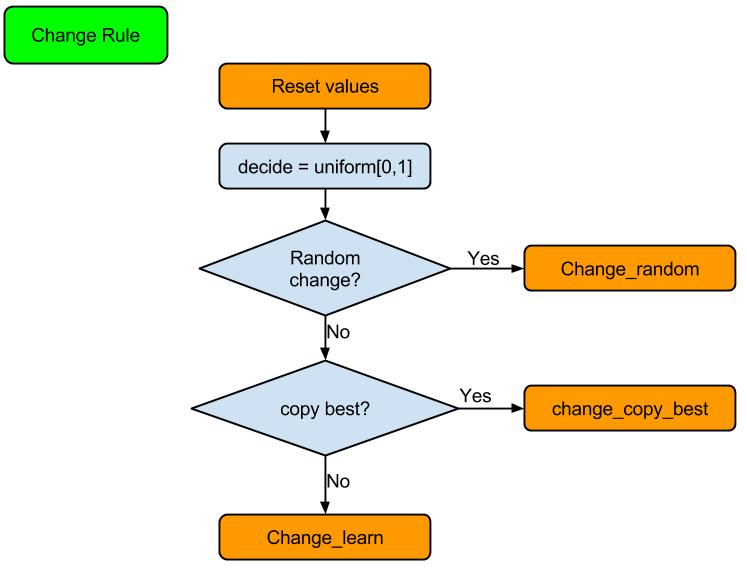
\includegraphics[width =\textwidth]{change_rule.jpg}
\caption{Change Rule}
\label{change_rule}
\end{figure}
\begin{alltt}
 \underline{\textit{Pseudo Code:}}
Reset values ;; see above 
let decide be a random number between 0 and 1
if (decide > 1 - random_change)
    Change_random
else
    change_copy_best
    else 
        Change_learn
\end{alltt}
\begin{figure}[!ht]
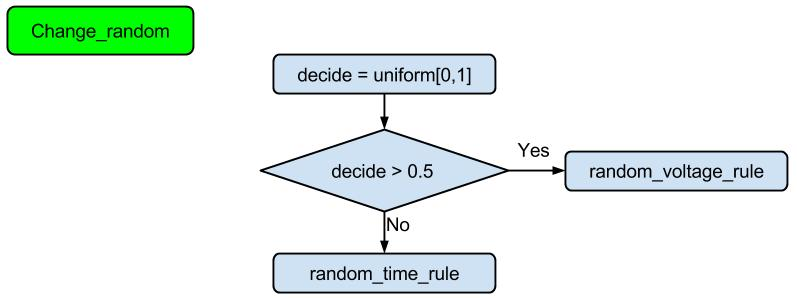
\includegraphics[width =\textwidth]{change_random.jpg}
\caption{Change random}
\label{change_random}
\end{figure}
\begin{figure}[!ht]
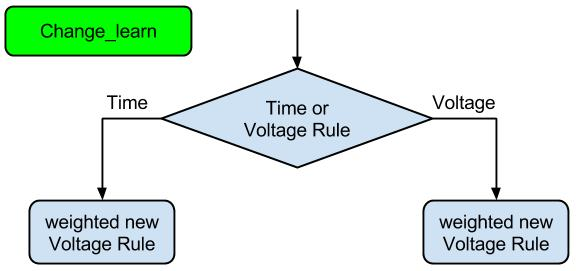
\includegraphics[width =\textwidth]{change_learn.jpg}
\caption{Change learn}
\label{change_learn}
\end{figure}

\begin{alltt}
 \underline{\textit{Pseudo Code:}}
let index = 0
let number_voltage be 0
let voltage_preference be 0
let number_time be 0
let time_preference be 0 
for k = 1 to 5 
    if (memory[k,1] == 1)
        set number_voltage = number_voltage + 1 
        set preference_voltage = preference_voltage + memory[k,7]
    if (memory[k,1] == 2)
        set number_time = number_time + 1 
        set preference_time = preference_time + memory[k,7]
    if (memory[k,1]==NA)
        set index to k - 1
if (index ==1)
    set active_rule to matrix[1, all]
else
    if (number_voltage==0 or number_time==0)
        if (number_voltage > number_time)
            set active_rule to weighted_new_voltage_rule
        else 
            set active_rule to weighted_new_time_rule
    else 
        if (preference_voltage/number_voltage > preference_time/number_time)
            set active_rule to weighted_new_voltage_rule
        else 
            set active_rule to weighted_new_time_rule

\underline{to report weighted_new_voltage_rule}
let averaged_rule be vector[0,0,0,0,0,0]
let count be 0
for k = 1 to 5 
    if (memory[k,1] == 1)
        averaged_rule = averaged_rule + memory[k, 1 to 6]
        count = count + 1 
return (averaged_rule  / count)

\underline{to report weighted_new_time_rule}
let averaged_rule be vector[0,0,0,0,0,0]
let count be 0
for k = 1 to 5 
    if (memory[k,1] == 2)
        averaged_rule = averaged_rule + memory[k, 1 to 6]
        count = count + 1 
return (averaged_rule  / count)
\end{alltt}

\begin{figure}[!ht]
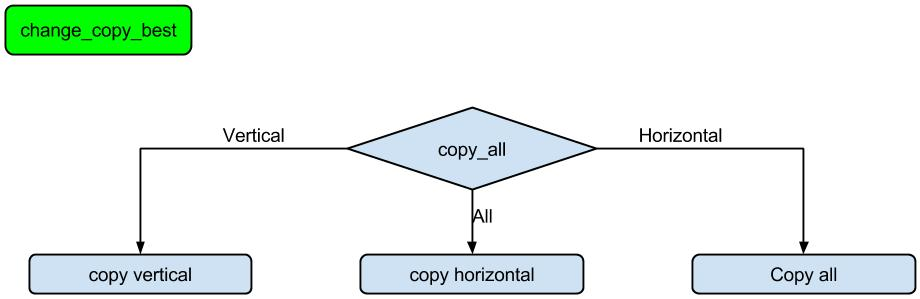
\includegraphics[width =\textwidth]{change_copy_best.jpg}
\caption{Change copy best}
\label{change_copy_best}
\end{figure}
\begin{alltt}
 \underline{\textit{Pseudo Code:}}
If copy_all = “all”
    let best_value be  -1
            let best_rule be empty rule
            for i in agents:
                if (node of i-th agent != node of original agent):
                        if preference of i-th best rule> best_value:
                            best_rule = best rule of i-th agent
                            best_value = preference of i-th agents best rule
            set active_rule  to  best_rule

elsif (copy_all == "vertical")
            let best_value be -1
            let best_rule be empty rule
            let branch be branch in which agent is in 
            for i in agents:
                let branch2 be branch in which  i-th agent is in  
                if ((branch == branch2) &(node of i-th agent != node of original agent)):
                        if preference of i-th best rule > best_value:
                                best_rule = best rule of i-th agent
                                best_value = preference of i-th agents best rule
            self.active_rule = best_rule
    else:
            let best_value be -1
            let best_rule be empty rule
            level = level of agent
            for i in agents:
                level2 = level on which i-th agent is on 
                if ((level == level2) & (node of i-th agent != node of original agent)):
                        if preference of i-th best rule > best_value:
                                best_rule = best rule of i-th agent
                                best_value = preference of i-th agents best rule
             set active_rule to  best_rule
\end{alltt}


\newpage
\begin{thebibliography}{9}

\bibitem{cprbook}
	Ostrom, E., Gardner, R., \& Walker, J. (1994). Rules, games, and common-pool resources. University of Michigan Press.
\bibitem{smartenergy}
	Lund, H., Andersen, A. N., Østergaard, P. A., Mathiesen, B. V., \& Connolly, D. (2012). 
	From electricity smart grids to smart energy systems–a market operation based approach and understanding. Energy, 42(1), 96-102.
\bibitem{smartcpr}
Wolsink, M. (2012). The research agenda on social acceptance of distributed generation in smart grids: Renewable as common pool 
resources. Renewable and Sustainable Energy Reviews, 16(1), 822-835.
\bibitem{disgust1}Stragier, J., Hauttekeete, L., \& De Marez, L. (2010, September). Introducing Smart grids in residential contexts: Consumers' perception of Smart household appliances. In Innovative Technologies for an Efficient and Reliable Electricity Supply (CITRES), 2010 IEEE Conference on (pp. 135-142). IEEE.
\bibitem{disgust2}Geelen, D., Reinders, A., \& Keyson, D. (2013). Empowering the end-user in smart grids: Recommendations for the design of products and services. Energy Policy, 61, 151-161.
\bibitem{disgust3} Park, C. K., Kim, H. J., \& Kim, Y. S. (2014). A study of factors enhancing smart grid consumer engagement. Energy Policy, 72, 211-218.
\bibitem{ethics1}Kostyk, T., \& Herkert, J. (2012). Societal implications of the emerging smart grid. Communications of the ACM, 55(11), 34-36.
\bibitem{ethics2}Fhom, H. S., \& Bayarou, K. M. (2011, November). Towards a holistic privacy engineering approach for smart grid systems. In Trust, Security and Privacy in Computing and Communications (TrustCom), 2011 IEEE 10th International Conference on (pp. 234-241). IEEE.
\bibitem{moneycant}Sandel, M. J. (2000). What money can't buy: the moral limits of markets. Tanner Lectures on Human Values, 21, 87-122.
\bibitem{smarthome}
Pedrasa, M. A. A., Spooner, T. D., \& MacGill, I. F. (2010). Coordinated scheduling of residential distributed energy resources to optimize smart home energy services. 
Smart Grid, IEEE Transactions on, 1(2), 134-143.
\bibitem{v2g}
Fattori, F., Anglani, N., \& Muliere, G. (2014). Combining photovoltaic energy with electric vehicles, smart charging and vehicle-to-grid. Solar Energy, 110, 438-451.
\bibitem{realtime}
Deilami, S., Masoum, A. S., Moses, P. S., \& Masoum, M. A. (2011). Real-time coordination of plug-in electric vehicle charging in smart grids to minimize power losses and 
improve voltage profile. Smart Grid, IEEE Transactions on, 2(3), 456-467.
\bibitem{ACDC}
Shaaban, M. F., Eajal, A. A., \& El-Saadany, E. F. (2014). Coordinated charging of plug-in hybrid electric vehicles in smart hybrid AC/DC distribution systems. Renewable Energy.
\bibitem{eth}
Galus, M. D., \& Andersson, G. (2008, November). Demand management of grid connected plug-in hybrid electric vehicles (PHEV). 
In Energy 2030 Conference, 2008. ENERGY 2008. IEEE (pp. 1-8). IEEE.
\bibitem{reinforce_money}
Valogianni, K., Ketter, W., \& Collins, J. (2013, July). Smart Charging of Electric Vehicles using Reinforcement Learning. In AAAI Workshop: Trading Agent Design and Analysis.
\bibitem{qfail}
Lauer, M., \& Riedmiller, M. (2000). An algorithm for distributed reinforcement learning in cooperative multi-agent systems. 
In In Proceedings of the Seventeenth International Conference on Machine Learning.
\bibitem{ai_cpr}Turner, R. M. (1993). The tragedy of the commons and distributed AI systems. Department of Computer Science, University of New Hampshire.
\bibitem{institutions}Tajima, K. (2007). The theory of institutions and collective action in Adam Smith's Theory of Moral Sentiments. The Journal of Socio-Economics, 36(4), 578-594.
\bibitem{machine}Alpaydin, E. (2014). Introduction to machine learning. MIT press.
\bibitem{multiagent}Vlassis, N. (2007). A concise introduction to multiagent systems and distributed artificial intelligence. Synthesis Lectures on Artificial Intelligence and Machine Learning, 1(1), 1-71.
\bibitem{matpower}R. D. Zimmerman, C. E. Murillo-Sanchez, and R. J. Thomas, \
Matpower: Steady-State Operations, Planning and Analysis Tools for Power Systems Research and Education,"
Power Systems, IEEE Transactions on, vol. 26, no. 1, pp. 12-19, Feb. 2011
\bibitem {powertransfer}\url{http://www.powerworld.com/files/S01SystemModeling.pdf}
\bibitem{mas}Wooldridge, M. (2009). An introduction to multiagent systems. John Wiley \& Sons.
\bibitem{cabletable}\url{http://ffcpg.com.my/portal/Products.nsf/2d248e16d8d12df4825719b00301d50/5801a1bfde86e113482577e40009d126/FILE/LV+TD.pdf}
\bibitem{ev_stakeholder}Bakker, S., Maat, K., \& Van Wee, B. (2014). Stakeholders interests, expectations, and strategies regarding the development and implementation of electric vehicles: The case of the Netherlands. Transportation Research Part A: Policy and Practice, 66, 52-64.
\bibitem{social_smart_grid}Skopik, F. (2014). The social smart grid: Dealing with constrained energy resources through social coordination. Journal of Systems and Software, 89, 3-18.
\bibitem{powerbook}Willis, H. L. (1997). Power Distribution Planning Reference Book. CRC Press.
\end{thebibliography}


\begin{comment}
\subsection{EV smart charging}
A standard low voltage grid with varying load profiles is used as a base model in MATPOWER. The load profiles resemble the average household electricity usage in 15 minute time intervals. On top of this base load each household has one electric vehicle(EV). Each EV has a specific battery size, a state of charge (SOC) and can be charged at different rates. Based on the combined load applied at each grid node MATPOWER calculates the voltage at each grid point. \\
Each agent manages one EV over a certain time horizon. The management is a markov decision process and the behavior of the agent is optimized using Q-learning. The state the agent is in is the SOC of the battery and the voltage at the grid point of the household. The action that the agent can take is to charge the EV at different rates within the next time step. This has an effect on the SOC and adds load to the grid point increasing the voltage deviation. The reward the agent receives is a function of the SOC of the battery and the voltage of the grid node. The higher the SOC the higher the reward, the higher the Voltage deviation from the norm the lower the reward. This way the agent has to balance the positive effect his action has on his state of charge with the negative effects his actions has on the voltage.\\
\begin{enumerate}
\item State\begin{enumerate}
\item SOC
\item Voltage
\end{enumerate}
\item Action\begin{enumerate}
\item Charge EV [0,5]kW
\item (Vote to change Reward function
\end{enumerate}
\item Reward\begin{enumerate}
\item $f(Voltage,SOC)=g(Voltage)+h(SOC)$
\end{enumerate}
\end{enumerate}
The effect the voltage deviation has on the reward function is what the agents collectively vote on. The agents vote on how strongly overuse of the grid should be penalized. This way the agents not just interact with the environment but also shape the environment.  
\begin{figure}
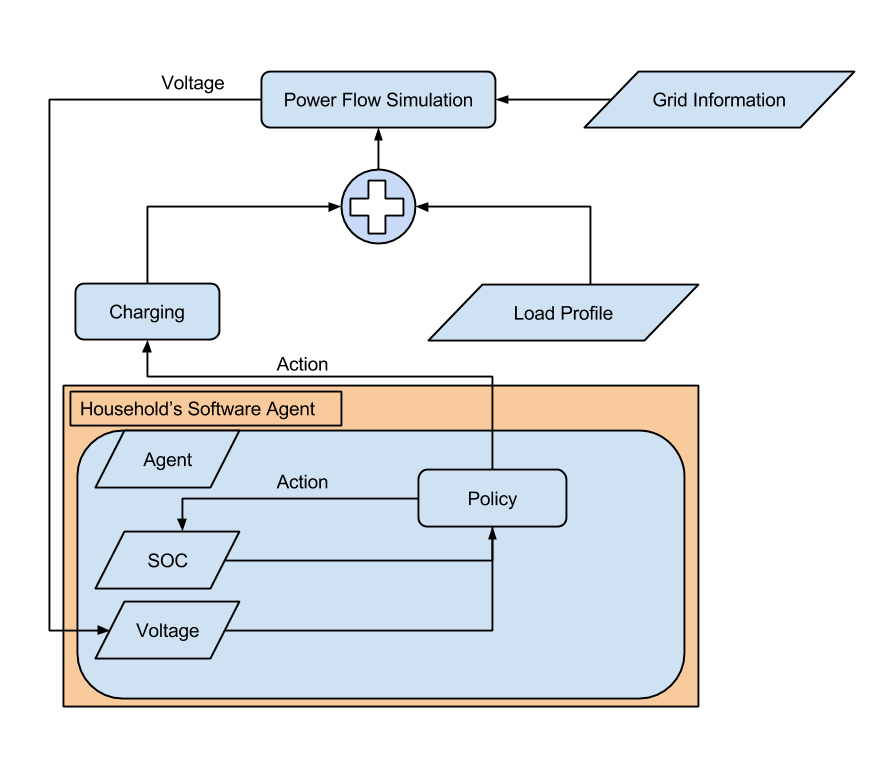
\includegraphics[width =\textwidth]{EV_smart_charging_model.pdf}
\caption{Smart charging Model}
\label{smartcharginggraph}
\end{figure}

\subsection{Experiment}
In order to answer the question with this model a congested situation has to be created, and how well the proposed algorithm deals with the situation will be observed.\\ 
Whether or not a situation is congested, will be determined by whether or not the voltage deviation at each grid point is within a predetermined voltage bandwidth. The case will have a base household load so that at peak load the voltage deviation is still within the voltage bandwidth, however when adding the uncontrolled charging profile of the electric vehicles to the household loads the voltage deviation exceeds the voltage bandwidth. This way a situation is created in which the grid is sufficient for normal household load but is overwhelmed if electric vehicles are introduced.\\ 
The agent will then learn best charging strategies by Q-learning and adapt the reward function to push the peak voltage deviation back into the voltage bandwidth. The hypothesis will be accepted if the agents are able to regulate each other and come up with rules to distribute the load from more congested to less congested situation and thus stabilize the grid.\\
%\begin{figure}[!ht]
%\includegraphics[width = \textwidth]{thesis_defense.png}
%\caption{Conclusion}
%\label{conclusion}
%\end{figure}

\newpage
\newpage
\newpage
\end{comment}


\end{document}